\documentclass{article}

\PassOptionsToPackage{numbers, compress}{natbib}
\usepackage[preprint,nonatbib]{neurips_2025}

\usepackage[utf8]{inputenc}
\usepackage[T1]{fontenc}
\usepackage{lmodern}
\usepackage{amsmath, amssymb}
\usepackage{graphicx}
\usepackage{longtable, booktabs}
\usepackage{array}
\usepackage{microtype}
\usepackage{url}
\usepackage[dvipsnames]{xcolor}
\usepackage[
  colorlinks=true,
  citecolor=NavyBlue,
  linkcolor=NavyBlue,
  urlcolor=NavyBlue
]{hyperref}
\usepackage[font=small,labelfont=bf]{caption}

% pandoc helpers
\providecommand{\tightlist}{\setlength{\itemsep}{0pt}\setlength{\parskip}{0pt}}
\providecommand{\pandocbounded}[1]{#1}

% csl bibliography (pandoc-citeproc)
\newlength{\cslhangindent}
\setlength{\cslhangindent}{1.5em}
\newlength{\csllabelwidth}
\setlength{\csllabelwidth}{3em}
\newenvironment{CSLReferences}[2]
 {%
  \setlength{\parindent}{0pt}
  \everypar{\setlength{\hangindent}{\cslhangindent}}\ignorespaces
 }
 {\par}

\title{A Comprehensive Survey of World Models for Coding}

\author{Keon Kim}

\date{May 2026}

\begin{document}

\maketitle


{\hypersetup{linkcolor=black}
\setcounter{tocdepth}{2}
\tableofcontents
}

\hypertarget{a-comprehensive-survey-of-world-models-for-coding}{%
\section{A Comprehensive Survey of World Models for
Coding}\label{a-comprehensive-survey-of-world-models-for-coding}}

\emph{Last updated 2026-05}

\begin{quote}
\textbf{Genre note.} This document is a hybrid: §§6--16 are a
conventional survey of the field (foundations, lineages, benchmarks,
empirical landscape), while §17 is an explicitly argumentative critical
synthesis. Readers who want only the catalog can skip §17; readers who
want only the criticism can read the Theses Summary below plus §17 and
skip §§6--16. The two halves are meant to be read together --- neither
alone captures the field's current shape.
\end{quote}

\begin{center}\rule{0.5\linewidth}{0.5pt}\end{center}

\hypertarget{abstract}{%
\subsection{Abstract}\label{abstract}}

A \emph{world model} is an internal predictor an agent maintains over
the dynamics of its environment, used to imagine the consequences of
actions. In coding, the environment is the program itself --- its
runtime state, its execution trace, the filesystem it manipulates, the
tests it must satisfy, the developer task it is solving. Twelve years
after Zaremba \& Sutskever asked whether a network could execute code
(Zaremba and Sutskever 2014), and seven months after Meta FAIR released
CWM (team et al. 2025) as the first openly-released LLM explicitly
branded a Code World Model, the question has changed. It is no longer
controversial that internal models of execution are \emph{learnable};
whether they are \emph{necessary}, \emph{architecturally separable}, or
\emph{causally responsible} for coding-agent gains remains unsettled.
The open questions are whether the \emph{named artifact} ``code world
model'' is a structural commitment or a marketing label, whether trace
pretraining buys what it claims, and whether the field's Dreamer-shaped
vocabulary will survive when the empirical evidence comes in.

This survey synthesizes 184 papers around the world-model lens. We
define the object of study with two distinct definitions --- a
permissive \emph{descriptive} one (what the field currently calls a code
WM) and a strict \emph{normative} one (architectural commitment to
forward state prediction); trace its twelve-year arc; build a three-axis
taxonomy (functionality × temporal × representation); produce technical
system cards for thirteen representative systems; assemble
protocol-stratified benchmark tables for SWE-bench, CRUXEval, web
agents, and formal verification; develop seven critical theses where the
field overclaims; and identify the open problems where new work would
matter most. The single most defensible empirical claim is that
\emph{execution-grounded supervision improves code agents on
runtime-reasoning-heavy benchmarks}; the single most defensible critical
claim is that broader inferences from this to ``world models in coding''
remain underdetermined by the evidence at this date.

\begin{center}\rule{0.5\linewidth}{0.5pt}\end{center}

\hypertarget{theses-summary-read-first}{%
\subsection{Theses Summary (Read
First)}\label{theses-summary-read-first}}

The survey is a hybrid: catalog plus critique. Readers pressed for time
can read this summary and §17 (Critical Perspectives) and skip the
lineage chapters (§§6--14). Readers entering the field should read
§§1--5 first, then §§6--16, then §17. The catalog and the critique are
meant to be read together.

The seven critical theses developed in §17, each grounded in a specific
disconfirmation from the corpus:

\begin{enumerate}
\def\labelenumi{\arabic{enumi}.}
\item
  \textbf{The ``world model'' label has become overloaded.} Under the
  field's permissive descriptive definition (D, §3.1), CWM, TRACED,
  SemCoder, LLM-JEPA, and DyMo are all ``world models'' despite being
  architecturally standard LLMs with enriched training. A strict
  normative definition (N1/N2/N3, §3.1) admits only systems with
  explicit forward-prediction machinery: neural dynamics models (N1, no
  code exemplar), latent-action rollout models such as CoLA (N2), and
  synthesized executable simulators such as GIF-MCTS and ARC executable
  WMs (N3).
\item
  \textbf{Trace pretraining has a causal-isolation problem.} ``Do Code
  Semantics Help?'' (J. Wang et al. 2025) finds no trace representation
  consistently improves code synthesis across multiple backbones; CWM's
  65.8\% SWE-bench Verified is confounded between trace mid-training,
  ForagerAgent trajectories, and RL.
\item
  \textbf{The Dreamer-for-code gap may be a non-problem.} Vision needed
  latent rollouts because pixels are expensive; Python state is small
  and CPython is free, so the architectural pressure does not transfer.
  CWM in token space reaches state-of-the-art at 32B.
\item
  \textbf{PRMs are critics, not world models.} A learned evaluator of
  partial trajectories cannot roll out future states; the conceptual
  conflation dilutes the world-model vocabulary.
\item
  \textbf{``General Agents Contain World Models'' (Richens et al. 2025)
  is weaker than its title.} The theorem applies under restrictive
  assumptions (full observability, stationarity, deep-composite-goal
  regret bounds) that SWE agents demonstrably violate.
\item
  \textbf{The verifier-grounded lineage is the actual leading edge, but
  scoped.} ATLAS, Re:Form, CLEVER, VeriStruct, AutoRocq produce
  machine-checkable correctness. Scoped: they lead on
  synthesis-from-spec (e.g., ATLAS DafnySynthesis 65.8\% pass@5); they
  do \emph{not} lead on end-to-end verified codegen from NL (CLEVER
  ≤1/161 Lean).
\item
  \textbf{The evaluation gap is the structural reason the field looks
  confused.} No benchmark holds policy fixed and varies WM quality.
  Models with 85--98\% output-prediction accuracy still produce traces
  with systematic errors throughout --- outcome accuracy decouples from
  process fidelity.
\end{enumerate}

These theses are the survey's main contribution. §§6--16 catalog the
work; §§16--17 provide the empirical and critical synthesis that grounds
the theses; §18 lists open problems.

\begin{center}\rule{0.5\linewidth}{0.5pt}\end{center}

\hypertarget{introduction}{%
\subsection{1. Introduction}\label{introduction}}

Autoregressive code LLMs generate tokens conditioned on syntactic
context. Correct programs live in two worlds: a \emph{syntactic} world
of tokens and a \emph{semantic} world of values, control flow, side
effects, and developer intent. The world-model framing --- imported from
model-based reinforcement learning, where it names an internal predictor
of environment dynamics used to imagine action outcomes --- is the
field's bet that the gap between these two worlds closes when the
network has been trained on what code does rather than only on what code
looks like.

Two adjacent surveys cover non-overlapping ground. \textbf{A Survey on
LLMs for Code Generation} (Jiang et al. 2024) maps the code-LLM space
without the world-model lens. \textbf{Understanding World or Predicting
Future} (J. Ding et al. 2024) maps world models in general without the
code lens. \textbf{A Comprehensive Survey on World Models for Embodied
AI} (X. Li et al. 2025) maps embodied world models but excludes the
coding domain. The intersection --- the subject of this document --- has
cohered only recently into a recognizable program.

We aim for three things at once: comprehensive coverage of the corpus,
technical depth on the canonical systems, and an honest accounting of
where the prevailing rhetoric outruns the evidence. The first two are
owed to readers entering the field; the third is owed to those already
in it.

\begin{center}\rule{0.5\linewidth}{0.5pt}\end{center}

\hypertarget{methodology}{%
\subsection{2. Methodology}\label{methodology}}

\textbf{Corpus construction.} The 184-PDF corpus enumerated in
\texttt{papers.json} was assembled in four iterative passes between
March and May 2026. The seed paper was CWM (team et al. 2025). Each pass
expanded the corpus along a different axis: (i) snowball search on cited
and citing papers via Semantic Scholar's reference API and arxiv
listings; (ii) targeted topic searches on subdomains where the previous
pass was thin (latent-action WMs for LLMs; safety/malicious-code;
symbolic-execution and formal verification; agent memory; REPL-grounded
models); (iii) a 2026-specific sweep to capture papers the earlier
passes missed because of arxiv-ID ambiguity; (iv) a focused fourth pass
on reasoning models, process reward models, test-generation,
decompilation, diffusion code models, mech-interp, ARC synthesis,
self-improvement, Verilog/RTL, and major 2026 capstones. Each pass
produced a written rationale for accepted and rejected candidates.

\textbf{Inclusion criteria.} A paper was included if it credibly
intersected \emph{both} (a) world-modeling, state-tracking, or
environment-prediction architectures, and (b) code generation,
debugging, repair, or agentic coding. Pure code-LLM papers without a
world-model angle and pure world-model papers without a code angle were
excluded. Where the boundary was ambiguous, we erred on the side of
inclusion when the paper introduced a representation, training
objective, or evaluation that could plausibly be adopted by code-WM
work.

\textbf{Exclusion criteria.} Excluded: pure transformer scaling papers;
pure vision world models (DreamerV1/V2/V3, V-JEPA, Genie) except where
cited as architectural precedent; generic RL theory; classical PL
foundations; benchmark surveys without methodological contribution. We
retained DreamerV1--V3 as named citations in §11 because they ground the
latent-action discussion, but did not include their PDFs in the corpus.

\textbf{Date cutoff.} Papers with arxiv submission dates through
2026-05-15. Arxiv-ID format YYMM.NNNNN means IDs beginning 2601, 2602,
2603, 2604, 2605 are valid 2026 papers (Jan--May 2026), not
future-dated. An earlier survey pass mistakenly excluded these; the
fourth pass corrected the omission.

\textbf{Selection bias and reproducibility.} Two biases are explicit.
First, anglocentric arxiv-first selection --- we did not systematically
cover Chinese-language preprint servers, workshop proceedings without
arxiv copies, or industry technical reports. Second, recency bias ---
60\% of the corpus is from 2025 onward, reflecting the field's actual
growth curve but also our search recency. The full corpus is enumerated
in \texttt{papers.json} with arxiv IDs, titles, and filenames; readers
can regenerate the bibliography from this index.

\textbf{Sources reconciled with adjacent surveys.} We compared our
taxonomy and corpus against three awesome-list repositories
(knightnemo/Awesome-World-Models, JiahuaDong/Awesome-World-Models,
tsinghua-fib-lab/World-Model) and two prior surveys (Ding et al. (J.
Ding et al. 2024) on world models in general; Li et al. (X. Li et al.
2025) on world models for embodied AI). The three-axis taxonomy in §5 is
adapted from Li et al.~with code-specific representation classes added.
Where our judgment diverges from these adjacent works --- for example,
in our classification of CWM as architecturally a token-policy rather
than a world-model proper (§17.1) --- we mark the divergence explicitly.

\textbf{Taxonomy coding.} Each paper was assigned at least one lineage
label (§§6--13) and at least one representation label (§5.3 table). The
assignments were made by one of us and are recorded in the per-section
enumerations and \texttt{README.md}. We have not yet performed
inter-rater reliability checks; readers should treat the assignments as
one curator's best judgment, not consensus.

\textbf{Search procedure (for reproducibility).} Seed: (team et al.
2025). Search engines: arxiv listing API (cs.SE, cs.PL, cs.LG, cs.CL
submission categories), Semantic Scholar Graph API
(\texttt{/paper/arXiv:\{id\}/references} and
\texttt{/paper/arXiv:\{id\}/citations},
fields=title,externalIds,abstract,year), and WebSearch with query
variants enumerated below. Date cutoff: arxiv submissions through
2026-05-15.

Representative search queries used across the four passes
(non-exhaustive): - ``world model code generation,'' ``code world
model'' - ``neural code execution,'' ``learning to execute'' -
``execution trace pretraining LLM,'' ``trace-aware code model'' -
``Dreamer code,'' ``JEPA LLM,'' ``latent action LLM'' - ``SWE agent
reinforcement learning,'' ``agentic coding world model'' -
``self-debugging execution simulation,'' ``trace-driven program repair''
- ``symbolic execution LLM,'' ``verified code generation Dafny,'' ``Lean
code agent'' - ``diffusion code model,'' ``decompilation LLM semantic
equivalence'' - ``Verilog RL world model,'' ``ARC executable world
model'' - ``process reward model code,'' ``long-CoT code reasoning''

\textbf{Inclusion / exclusion counts.} Pass 1 considered
\textasciitilde70 candidates, accepted 31. Pass 2 considered
\textasciitilde40, accepted 20 (focused on 2026 papers earlier passes
missed). Pass 3 considered \textasciitilde80, accepted 52 via citation
BFS from 11 central papers. Pass 4 considered \textasciitilde60,
accepted 28 across 5 thin niches. Final corpus: 184 PDFs (one was added
late: (X. Li et al. 2025)). Total candidates considered:
\textasciitilde250. Rejection reasons recorded per-paper in the pass
reports.

\textbf{Limitations of this methodology.} Four. (1) No formal
inter-rater reliability metric --- one curator did the taxonomy coding.
(2) No systematic verification of the headline numerical claims in every
cited paper; §16 numbers were verified by reading the source PDFs but
§§7--14 inline claims rely on abstracts and our prior reading. (3) The
corpus is unstable --- between drafts several 2026 papers we initially
excluded as off-topic turned out to be relevant. A fifth pass would
change the count by ±15 papers without materially changing the survey's
conclusions. (4) Selection bias toward arxiv-first, anglophone,
code-LLM-adjacent sources; we did not systematically cover
Chinese-language preprint servers, workshop proceedings without arxiv
copies, or industry technical reports.

\begin{center}\rule{0.5\linewidth}{0.5pt}\end{center}

\hypertarget{defining-a-world-model-for-coding}{%
\subsection{3. Defining a World Model for
Coding}\label{defining-a-world-model-for-coding}}

The literature uses ``world model'' in two distinct senses that this
survey will carefully separate.

\hypertarget{two-definitions}{%
\subsubsection{3.1 Two definitions}\label{two-definitions}}

\textbf{Definition D (descriptive, permissive).} A \emph{world model for
coding} is any code LLM whose training objective concretely encodes
program semantics --- execution traces, runtime state, environment
feedback, or simulated outcomes --- in addition to or instead of
source-token prediction. This is the field's current usage. Under D,
CWM, TRACED, SemCoder, LLM-JEPA, DyMo, RLEF, and most papers in the
corpus are world models.

\textbf{Definition N (normative, strict).} A \emph{world model for
coding} is a system with an explicit, separable forward-prediction
mechanism. We split N into three sub-types:

\begin{itemize}
\tightlist
\item
  \textbf{N1 --- Neural dynamics model.} A learned
  \texttt{W\ :\ (state,\ action)\ →\ next\_state} instantiated as a
  distinct architectural component with latent recurrent state, separate
  dynamics head, or inverse model. Dreamer-class. No code exemplar in
  the corpus.
\item
  \textbf{N2 --- Latent-action model.} A learned action abstraction over
  a base LLM, with the LLM serving as transition model in compressed
  action space, supporting rollout or tree search over latent actions.
  CoLA (Jia et al. 2025) is the canonical example.
\item
  \textbf{N3 --- Synthesized executable simulator.} The world model is
  an executable program (Python, DSL) synthesized by an LLM and run
  against ground-truth transitions during planning. GIF-MCTS (Dainese et
  al. 2024), WorldCoder, Executable WMs for ARC-AGI-3 (Rodionov 2026).
\end{itemize}

Each N-subtype has a distinct architectural commitment. N1 commits to
learned latent dynamics; N2 commits to a discrete latent-action space;
N3 commits to program synthesis as the dynamics. Conflating them --- as
the loose ``Dreamer-for-LLMs gesture'' framing did --- obscures which
architectural bet is being made. Under any N-subtype, CWM, TRACED,
SemCoder, and most of the corpus do \emph{not} qualify.

The two definitions agree on the empirical fact that execution-grounded
supervision helps. They disagree on whether that grounding is correctly
named a \emph{world model} in the model-based-RL sense.

\begin{longtable}[]{@{}
  >{\raggedright\arraybackslash}p{(\columnwidth - 4\tabcolsep) * \real{0.33}}
  >{\raggedright\arraybackslash}p{(\columnwidth - 4\tabcolsep) * \real{0.33}}
  >{\raggedright\arraybackslash}p{(\columnwidth - 4\tabcolsep) * \real{0.33}}@{}}
\toprule
Aspect & Definition D (descriptive) & Definition N (normative) \\
\midrule
\endhead
Granted to & Any LLM trained with execution-related signal & Only
systems with explicit forward-prediction module \\
Includes CWM & Yes & No (architecturally a Llama-class decoder) \\
Includes TRACED, SemCoder, NExT & Yes & No (auxiliary heads on a
Transformer) \\
Includes CoLA, GIF-MCTS & Yes & Yes \\
Includes PRMs (ExecVerify, ThinkPRM) & Often grouped & No (critics, not
forward predictors) \\
Includes verifiers (Lean, Dafny, Z3) & Sometimes grouped & No
(deterministic oracles, not learned WMs) \\
Includes Dreamer / V-JEPA (vision precedents) & Yes & Yes \\
\bottomrule
\end{longtable}

This survey uses \textbf{D throughout the catalog sections (§§6--16)}
because that is how the literature talks, and \textbf{N in §17} because
the critical synthesis depends on it. We mark the switch each time it
matters. The split has been called for in prior reviews of the field and
the two-definition framework is, in our reading, the cleanest
resolution.

\hypertarget{what-is-modeled}{%
\subsubsection{3.2 What is modeled}\label{what-is-modeled}}

Orthogonal to D-vs-N, a fourth question asks \emph{what} is modeled. The
corpus splits across:

\begin{itemize}
\tightlist
\item
  variable values and stack frames (CWM, CodeExecutor)
\item
  linear or branching execution traces (NExT, SemCoder, TRACED)
\item
  test outcomes and runtime errors (LEVER, RLEF)
\item
  environment/OS/web state (WebDreamer, Dyna-Think)
\item
  repository state (RepoGraph, Understanding by Reconstruction)
\item
  developer task or specification (ATLAS, Re:Form)
\item
  adversarial behavior (Double Life of CWMs)
\end{itemize}

A given system typically commits strongly to one or two of these.

\hypertarget{behavioral-vs-architectural-classification}{%
\subsubsection{3.3 Behavioral vs architectural
classification}\label{behavioral-vs-architectural-classification}}

CWM occupies an instructive position. \emph{Behaviorally}, it emits
stack frames and variable bindings, which feels like an ``explicit
symbolic world model.'' \emph{Architecturally}, it is a 32B Llama-class
decoder with no separate dynamics head, RSSM, or inverse model. The two
readings are both correct: CWM is \textbf{behaviorally explicit but
architecturally implicit}. Earlier framings in the literature (and
earlier drafts of this survey) collapsed these into a single ``explicit
WM'' label; we recommend separating them. SemCoder, NExT, and TRACED
follow the same pattern.

\begin{center}\rule{0.5\linewidth}{0.5pt}\end{center}

\hypertarget{twelve-years-of-code-world-models}{%
\subsection{4. Twelve Years of Code World
Models}\label{twelve-years-of-code-world-models}}

The lineage is best understood as a sequence of inheriting questions.
Each era's answer dissolved the previous era's bottleneck and exposed
the next.

\begin{figure}
\centering
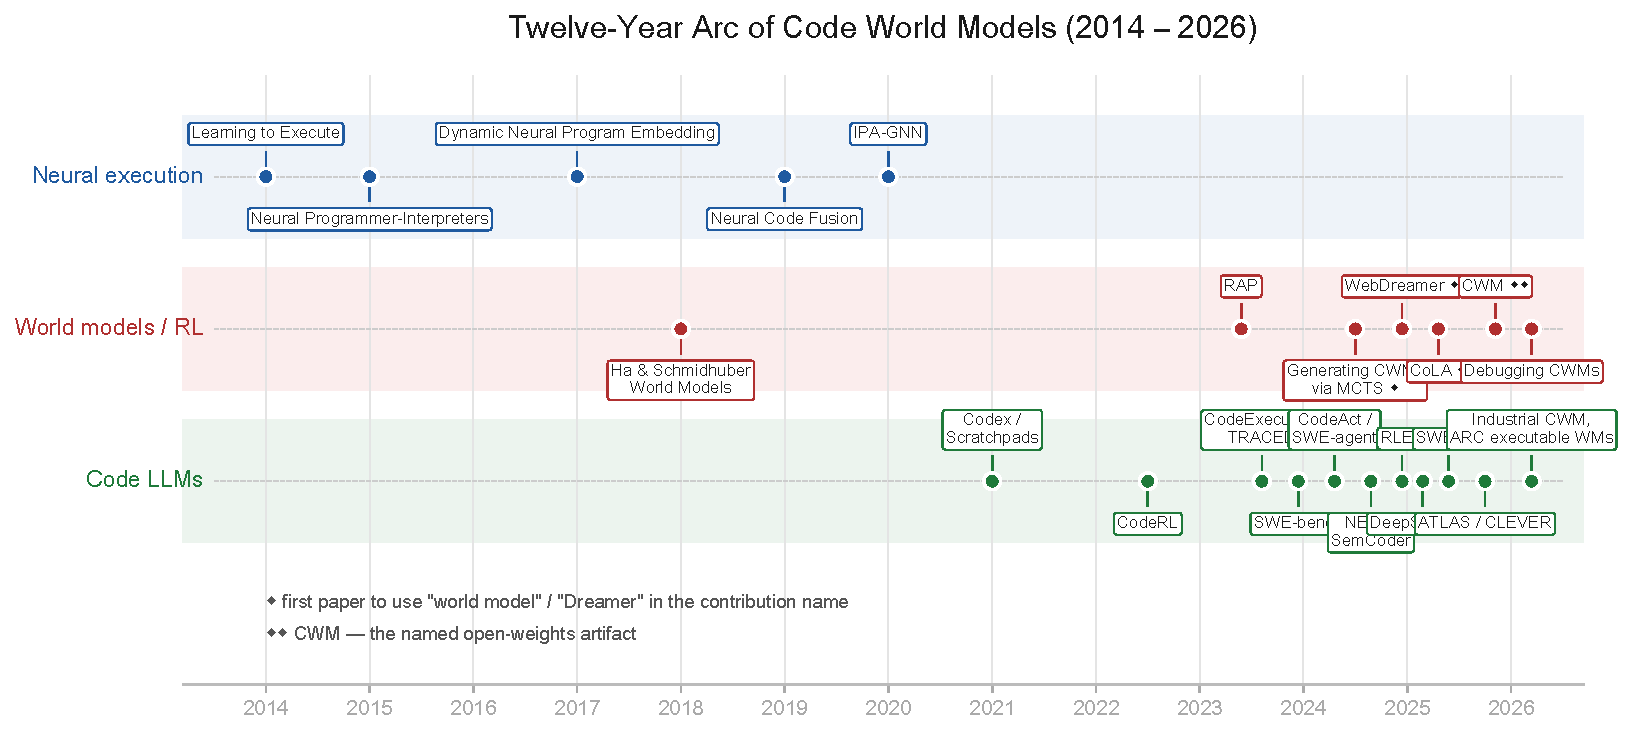
\includegraphics[width=1\textwidth,height=\textheight]{fig_timeline.pdf}
\caption{Twelve-year arc of code world models (2014--2026). Three
parallel lineages --- neural execution, world models / RL, and code LLMs
--- converge in 2025--2026 around the named artifact CWM. ◆ marks the
first paper to use ``world model'' / ``Dreamer'' in a contribution name;
◆◆ marks CWM as the named open-weights artifact.}
\end{figure}

Diamonds (◆) mark moments where ``world model'' enters the \emph{name}
of the contribution.

\textbf{Pre-2020 --- Can a network execute code?} Zaremba \& Sutskever's
\textbf{Learning to Execute} (Zaremba and Sutskever 2014) handed an LSTM
character-level Python and asked it to predict output. The model worked
on straight-line programs with bounded loops, but only with a curated
curriculum, and only because the LSTM's constant memory was just enough
to simulate the interpreter when the interpreter ran in constant memory
too. Everything that followed in this lineage tried to escape that
curse. \textbf{Neural Programmer-Interpreters} (Reed and Freitas 2015)
and the \textbf{Differentiable Forth Interpreter} built differentiable
program counters and call stacks --- the bet that the right architecture
would close the gap. \textbf{Dynamic Neural Program Embedding} (K. Wang,
Singh, and Su 2017) made the inverse move: run the real interpreter,
embed the resulting state traces. \textbf{Neural Code Fusion} (Shi et
al. 2019) and \textbf{IPA-GNN} (Bieber et al. 2020) extended the
GNN-over-execution playbook to the point where attention played the role
of the program counter. By 2020 the lineage had answered its question
--- yes, a neural network can play interpreter, but only when the
interpreter is encoded into its architecture, and these architectures
did not transfer to Python, C, or assembly at corpus scale. Ha \&
Schmidhuber's \textbf{World Models} paper (Ha and Schmidhuber 2018) had
already named for vision and RL exactly the pattern this lineage was
reaching for. The vocabulary existed; the coding community had not yet
borrowed it.

\textbf{2020--2022 --- Can the network's training include execution?}
The era's reframing was simple: instead of \emph{can the network
execute}, ask \emph{can we train a normally-shaped Transformer on enough
execution evidence that semantics seep into its weights}. \textbf{Codex}
(M. Chen et al. 2021) and \textbf{MBPP} (Austin et al. 2021) made code
generation a real engineering target. \textbf{Show Your Work /
Scratchpads} (Nye et al. 2021) made the decisive move: a Transformer
that could not predict a program's output could predict it perfectly if
it was allowed to emit the intermediate computation first. Same trick
Dynamic Neural Program Embedding had pulled, now at LLM scale, in token
space, without architectural surgery. The neural-as-interpreter program
of 2014--2020 did not scale beyond toy languages; the next era's move
was to bake execution into training data rather than architecture.

\textbf{2023 --- Trace pretraining as a named recipe.}
\textbf{CodeExecutor} (C. Liu et al. 2023) made the recipe explicit:
mutate competitive-programming submissions, run them in a sandbox,
capture per-line state tokens, train a transformer to emit the trace
from source. \textbf{TRACED} (Y. Ding et al. 2023) generalized this to a
pretraining auxiliary that any code-LLM could absorb. \textbf{CRUXEval}
(A. Gu et al. 2024) provided the canonical input/output-prediction
benchmark and suddenly there was a number that captured ``does this
model understand what code does, as opposed to what code looks like.''
In parallel, \textbf{Reflexion} (Shinn et al. 2023) and
\textbf{Self-Debug} (X. Chen et al. 2023) showed that an LLM's mistakes
could be fed back to itself as natural-language critiques,
\textbf{LEVER} (Ni et al. 2023) used execution to verify candidate
generations during decoding, and \textbf{RAP} (Hao et al. 2023) framed
the LLM itself as a world model and ran MCTS over its imagined rollouts.
The year's unifying insight: execution traces are an auxiliary
objective, not a separate model.

\textbf{2024 --- From models that simulate to agents that act.}
\textbf{SWE-bench} (Jimenez et al. 2023) replaced ``write a function
that passes a unit test'' with ``fix a real GitHub issue in a real
repository.'' \textbf{CodeAct} (X. Wang et al. 2024) claimed the agent's
action space should be Python code itself. \textbf{SWE-agent} (John Yang
et al. 2024) shipped the harness. \textbf{NExT} (Ni et al. 2024) inlined
traces into the agent loop. \textbf{RLEF} (Gehring et al. 2024) fed
execution outcomes back as RL rewards. \textbf{WebDreamer} (Y. Gu et al.
2024) transplanted Dreamer-style imagination to digital agents.
\textbf{Generating Code World Models via MCTS} (Dainese et al. 2024)
introduced the literal phrase ``Code World Models.'' What unified the
year was a structural shift in \emph{where} the world model lives: in
2023 it lived in the weights, surfaced through trace prediction; in 2024
it lived in the loop, in the agent's behavior under environmental
feedback.

\textbf{2025 --- The CWM moment.} \textbf{DeepSeek-R1} (DeepSeek-AI et
al. 2025) opened the year by showing that pure reasoning-RL on
verifiable rewards could reach the frontier on math and code.
\textbf{SWE-RL} (Y. Wei, Duchenne, et al. 2025) applied the same recipe
to full SWE traces. \textbf{CoLA} (Jia et al. 2025) made the first
concrete attempt at a Dreamer-for-LLMs: inverse-dynamics over latent
actions, then RL over a learned codebook. \textbf{LLM-JEPA} (Huang,
LeCun, and Balestriero 2025) ported LeCun's joint-embedding predictive
objective to language. \textbf{General Agents Contain World Models}
(Richens et al. 2025) supplied a theorem: any agent satisfying a regret
bound on goal-conditioned tasks must have learned a predictive model of
its environment. Then in October, Meta FAIR released \textbf{CWM} (team
et al. 2025) --- a 32B open-weights model mid-trained on 5T tokens of
Python execution traces and ForagerAgent trajectories from Dockerized
repositories. The thing the 2014 LSTM was trying to be was now a
downloadable checkpoint.

\textbf{2026 --- Stress-testing and broadening.} With the artifact in
hand, the field pivoted to critique and generalization.
\textbf{Debugging Code World Models} (Rahmani 2026) catalogs CWM's
failures on long traces and string-state representation.
\textbf{Demystifying Errors in LLM Reasoning Traces} (Abdollahi et al.
2025) audits where trace-trained models hallucinate. \textbf{Industrial
CWM} (Jian Yang et al. 2026) and \textbf{Parallel-Code WMs} (Singh et
al. 2026) generalize the recipe to Verilog/GPU and parallelism
semantics. \textbf{Executable World Models for ARC-AGI-3} (Rodionov
2026) brings the generative-environment flavor to abstract visual
reasoning. \textbf{Reinforcement World Model Learning for LLM Agents}
(Yu et al. 2026) flips the standard recipe by training the WM rather
than the policy.

\textbf{The arc.} Across twelve years: \emph{can a network execute
code?} → \emph{can a network's training include execution?} → \emph{can
an LLM agent simulate its environment?} → \emph{is the world model a
named artifact rather than a metaphor?} Each era's answer dissolved the
previous bottleneck and exposed the next. Architecture gave way to data;
data gave way to agency; agency gave way to artifacts. What was a
half-philosophical question in 2014 --- \emph{does this network
understand what code does} --- became, in 2025, an operational one with
an open-weights baseline. The field has not finished. The 2026 critique
wave shows the artifact is brittle in ways the 2014 LSTM was never asked
to be. But the trajectory is now legible.

\begin{center}\rule{0.5\linewidth}{0.5pt}\end{center}

\hypertarget{taxonomy-three-axes-of-code-world-models}{%
\subsection{5. Taxonomy: Three Axes of Code World
Models}\label{taxonomy-three-axes-of-code-world-models}}

Two cuts at the taxonomy are useful, and they are complementary. The
first is a \emph{lineage} cut --- which research thread produced the
system --- and is the basis for §§6--13. The second, more durable cut
adapts the three-axis framework of Li et al.~((X. Li et al. 2025),
\emph{A Comprehensive Survey on World Models for Embodied AI}) to the
code domain. The lineage map is below; the three axes are developed in
§§5.1--5.3.

\begin{figure}
\centering
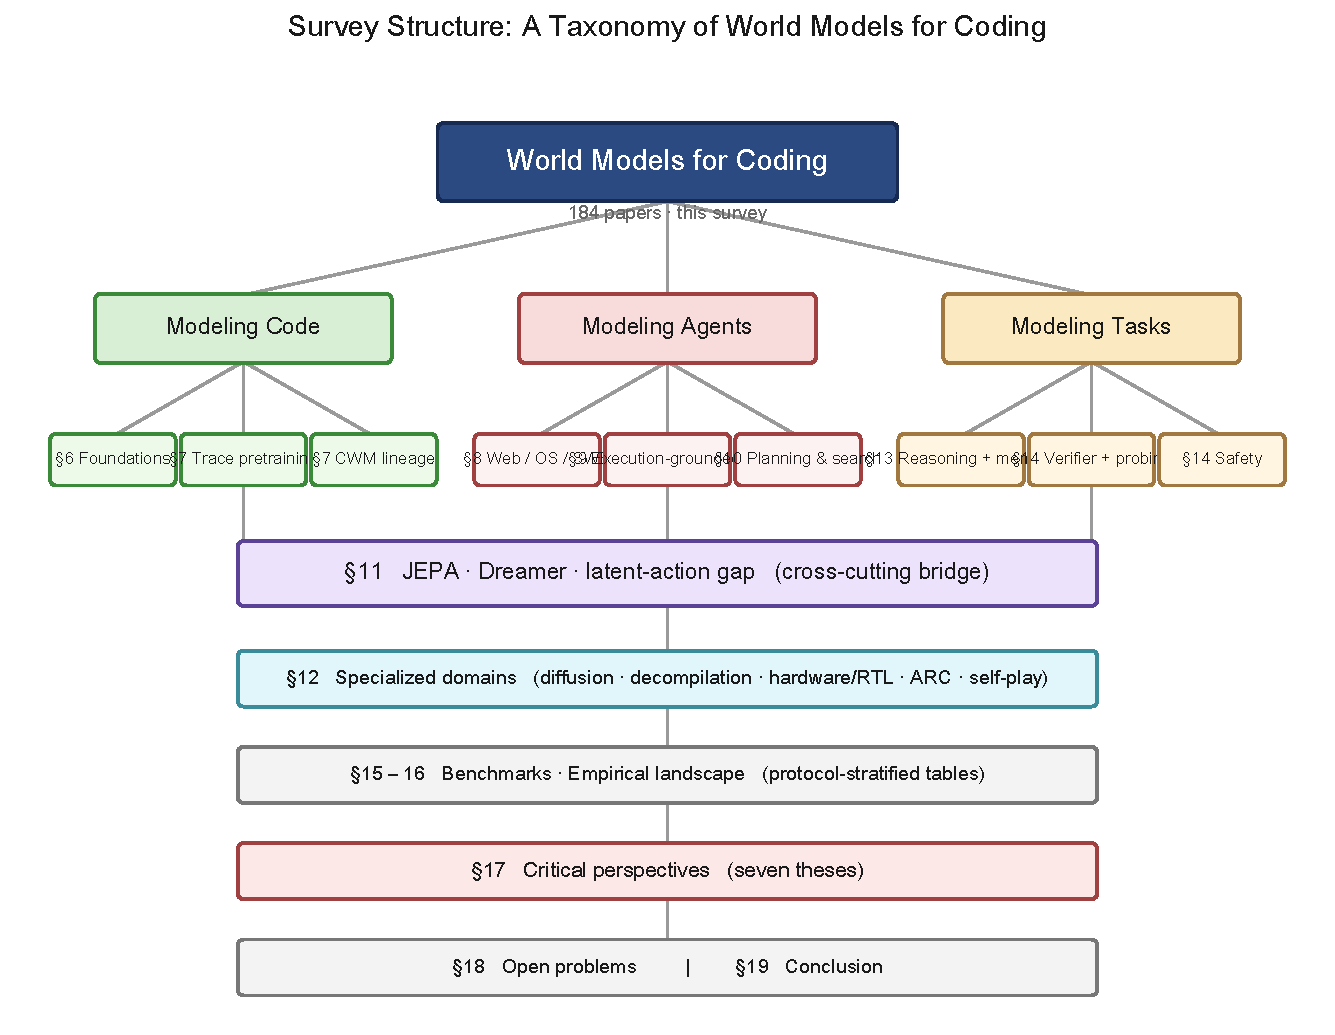
\includegraphics[width=1\textwidth,height=\textheight]{fig_taxonomy.pdf}
\caption{Taxonomy of world models for coding. The three primary modeling
axes (code, agents, tasks) are bridged by the JEPA / Dreamer /
latent-action discussion in §11. Specialized domains and synthesis
chapters sit below.}
\end{figure}

Adjacent WM surveys converge on overlapping splits that the three-axis
framework subsumes as projections. Ding et al. (J. Ding et al. 2024)
split top-level by \emph{implicit representation} vs \emph{future
prediction}. JiahuaDong's awesome-list organizes by \emph{paradigm}:
RL-based / observation-generative / latent-space / object-centric.
knightnemo's list surfaces \emph{pixel vs mesh vs latent} as
cross-cutting tags. The three axes --- functionality, temporal modeling,
and representation --- capture the choices a system makes regardless of
which lineage it belongs to.

\hypertarget{axis-1-functionality}{%
\subsubsection{5.1 Axis 1 ---
Functionality}\label{axis-1-functionality}}

\begin{itemize}
\tightlist
\item
  \textbf{Decision-coupled WMs} model only the slice of the world
  relevant to acting on it. CWM (team et al. 2025), RLEF (Gehring et al.
  2024), and WebDreamer (Y. Gu et al. 2024) are decision-coupled ---
  their WMs exist to enable code generation, RL planning, or web
  navigation respectively. CWM does not predict global filesystem state;
  it predicts the next Python frame \emph{because} the next action
  depends on it.
\item
  \textbf{General-purpose WMs} model the environment without reference
  to a particular task. The ``general agents contain world models''
  theorem (Richens et al. 2025) is the abstract limit. In the corpus,
  only the largest CWM-class models with broad mid-training approach
  generality; most ``code world models'' are decision-coupled to a
  sub-task (repair, completion, agent control).
\end{itemize}

\hypertarget{axis-2-temporal-modeling}{%
\subsubsection{5.2 Axis 2 --- Temporal
Modeling}\label{axis-2-temporal-modeling}}

\begin{itemize}
\tightlist
\item
  \textbf{Sequential simulation/inference.} Step-by-step autoregressive
  rollout. CWM, NExT, SemCoder, all the trace-pretraining systems, and
  most LLM-as-WM planners (RAP, WebDreamer in its MPC loop) live here.
  The state is updated one timestep at a time. The vision analog is RSSM
  (Hafner et al., DreamerV1--V3).
\item
  \textbf{Global difference prediction.} Predict the entire future state
  at once, in parallel. The vision analog is video-diffusion or
  masked-JEPA. In code, this fits diffusion code models (DiffuCoder,
  (Gong et al. 2025); Dream-Coder 7B, (Xie et al. 2025)) where the next
  state is sampled jointly rather than autoregressively, and the
  ``specification is the program'' framing (Monperrus 2026) where the
  entire trace is the spec.
\item
  \textbf{Static, no-trace.} Some systems (SemCoder's static mode, the
  trace-free baselines in ``Do Code Semantics Help?'') explicitly drop
  temporal modeling at inference, reducing to single-shot prediction.
\end{itemize}

\hypertarget{axis-3-representation}{%
\subsubsection{5.3 Axis 3 ---
Representation}\label{axis-3-representation}}

This is the axis where the WM literature has converged most strongly,
and where the code-WM literature is most uneven. Adapting Li et al.'s
four-category split (GLV / TFS / SLG / DRR) to code yields five classes,
of which only two are well-populated.

\begin{longtable}[]{@{}
  >{\raggedright\arraybackslash}p{(\columnwidth - 6\tabcolsep) * \real{0.25}}
  >{\raggedright\arraybackslash}p{(\columnwidth - 6\tabcolsep) * \real{0.25}}
  >{\raggedright\arraybackslash}p{(\columnwidth - 6\tabcolsep) * \real{0.25}}
  >{\raggedright\arraybackslash}p{(\columnwidth - 6\tabcolsep) * \real{0.25}}@{}}
\toprule
Class & Encodes the world as & Vision analog & Code exemplars \\
\midrule
\endhead
\textbf{Token Sequence (TS)} & Discrete or continuous token streams with
execution traces, variable bindings, or rationales interleaved with
source & Token-as-pixel (IRIS, TWM, Genie, Sora) & CWM (team et al.
2025), CodeExecutor (C. Liu et al. 2023), TRACED (Y. Ding et al. 2023),
NExT (Ni et al. 2024), SemCoder (Y. Ding et al. 2024) --- the dominant
code-WM mode \\
\textbf{Global Latent Vector (GLV)} & A compact vector updated
recurrently, encoding the entire program/agent state & RSSM (Hafner et
al., DreamerV1--V3) & \textbf{No clean exemplar.} CoLA (Jia et al. 2025)
introduces a learned action codebook but is otherwise a standard LLM,
not RSSM-style \\
\textbf{Spatial / Structural Grid (SLG)} & A geometric or structural
grid (BEV/voxel in vision; AST, call-graph, CFG in code) & OccWorld,
DriveWorld & \textbf{No exemplar.} RepoGraph (Ouyang et al. 2024) uses a
static dependency graph but does not predict over it as a WM \\
\textbf{Decomposed Object / Slot (DOR)} & Distinct persistent latent
slots for objects in the world & SlotFormer and object-centric WMs &
\textbf{No exemplar.} No code-WM models variables, scopes, or classes as
discrete persistent slots \\
\textbf{Synthesized executable (N3)} & The world model \emph{is} an
executable program, synthesized rather than learned & (orthogonal to
vision) & GIF-MCTS (Dainese et al. 2024), WorldCoder, Executable WMs for
ARC-AGI-3 (Rodionov 2026) \\
\bottomrule
\end{longtable}

Verifiers (Lean, Dafny, Z3) and PRMs are intentionally absent from this
table. A verifier is not a \emph{representation} of the world; it is a
\emph{grounding oracle} over candidate artifacts. A PRM is a
\emph{backward-looking critic}, not a forward predictor. Both belong in
§5.4 below.

\textbf{Three white spaces.} The Dreamer-style GLV, the object-centric
DOR, and the spatial-grid SLG representations have not been instantiated
for code, despite being mature for vision. §18 lists these as open
problems, with the caveat that not all three are equally promising ---
the Dreamer-style gap is contestable (§17.3), while the object-centric
and structural-grid gaps look more genuine.

\hypertarget{grounding-mode-orthogonal-to-representation}{%
\subsubsection{5.4 Grounding mode (orthogonal to
representation)}\label{grounding-mode-orthogonal-to-representation}}

A second classification asks how each system's predictions are
validated. This is the analog of Li et al.'s ``reality'' column and
addresses the decoupling between WM-head accuracy and downstream task
success that DyMo (Guo et al. 2025) and §17.7 develop.

\begin{longtable}[]{@{}
  >{\raggedright\arraybackslash}p{(\columnwidth - 4\tabcolsep) * \real{0.33}}
  >{\raggedright\arraybackslash}p{(\columnwidth - 4\tabcolsep) * \real{0.33}}
  >{\raggedright\arraybackslash}p{(\columnwidth - 4\tabcolsep) * \real{0.33}}@{}}
\toprule
Grounding mode & Definition & Code exemplars \\
\midrule
\endhead
None / self-report & Predictions never validated against ground truth &
RAP (Hao et al. 2023), basic LLM-as-WM planners \\
Execution-grounded & Predictions checked against real interpreter /
runtime & CWM (team et al. 2025), TRACED (Y. Ding et al. 2023), NExT (Ni
et al. 2024), SemCoder (Y. Ding et al. 2024), RLEF (Gehring et al.
2024) \\
Verifier-grounded & Outputs checked by Lean / Dafny / Verus / Rocq / Z3
& ATLAS (Baksys et al. 2025), Re:Form (C. Yan et al. 2025), CLEVER
(Thakur et al. 2025), VeriStruct (C. Sun et al. 2025), AutoRocq (Tu et
al. 2025) \\
Synthesized-simulator-checked & Synthesized world model checked against
held-out transitions & GIF-MCTS (Dainese et al. 2024), Executable WMs
for ARC-AGI-3 (Rodionov 2026) \\
Critic-grounded (not a WM) & Backward-looking value/quality score, no
rollout & ExecVerify (Tang et al. 2026), SWE-PRM (Gandhi et al. 2025),
ThinkPRM (Khalifa et al. 2025) --- listed for contrast; these are
critics, not WMs (§17.4) \\
\bottomrule
\end{longtable}

Grounding mode is orthogonal to the representation axis: a
token-sequence representation can be execution-grounded (CWM) or
self-report (RAP); an N3 synthesized-simulator can be checked against
transitions (GIF-MCTS) or never validated. The ``WM fidelity'' question
of §17.7 is, structurally, a question about whether a system's grounding
mode is strong enough to falsify a bad WM at training time.

\begin{center}\rule{0.5\linewidth}{0.5pt}\end{center}

\hypertarget{foundations-neural-execution-as-implicit-world-modeling}{%
\subsection{6. Foundations: Neural Execution as Implicit World
Modeling}\label{foundations-neural-execution-as-implicit-world-modeling}}

Zaremba \& Sutskever's \textbf{Learning to Execute} (Zaremba and
Sutskever 2014) established both feasibility and brittleness.
\textbf{Show Your Work --- Scratchpads} (Nye et al. 2021) is the hinge
moment: by training a Transformer to emit intermediate computation
states, the authors recovered much of the LSTM-era execution-prediction
performance at scale, presaging the trace-pretraining lineage of §6.
\textbf{CRUXEval} (A. Gu et al. 2024) and \textbf{REval} (J. Chen et al.
2024) provide the canonical execution-reasoning benchmarks. The lesson
the field absorbed: \emph{replacing} the interpreter with a neural
network is harder than \emph{augmenting} a transformer with
interpreter-style supervision. Modern systems all take the latter path.

\begin{center}\rule{0.5\linewidth}{0.5pt}\end{center}

\hypertarget{the-trace-pretraining-and-cwm-lineage}{%
\subsection{7. The Trace-Pretraining and CWM
Lineage}\label{the-trace-pretraining-and-cwm-lineage}}

\hypertarget{trace-pretraining-as-a-recipe}{%
\subsubsection{7.1 Trace-pretraining as a
recipe}\label{trace-pretraining-as-a-recipe}}

\textbf{CodeExecutor} (C. Liu et al. 2023) trains a Transformer to
simulate Python execution token-by-token. \textbf{TRACED} (Y. Ding et
al. 2023) adds dynamic-state supervision to a code-LLM pretraining mix.
\textbf{NExT} (Ni et al. 2024) formats traces as natural-language
rationales, letting a chat-style LLM reason about runtime behavior via
chain-of-thought. \textbf{SemCoder} (Y. Ding et al. 2024) generalizes to
``monologue reasoning'' linking source-text to execution state.

The 2025 wave consolidated and stress-tested the approach.
\textbf{``What I cannot execute, I do not understand''} (Armengol-Estapé
et al. 2025) trains and evaluates LLMs explicitly on traces with dynamic
scratchpads, pushing Llama-3.1-8B from 37.8\% to \textasciitilde80\% on
CRUXEval-O. \textbf{Code Execution as Grounded Supervision} (Jung, Zhou,
and Chen 2025) repurposes line-by-line traces as verifiable CoT.
\textbf{Self-Execution Simulation} (Maimon et al. 2026) lets the model
train on its own execution predictions. \textbf{Demystifying Errors in
LLM Reasoning Traces} (Abdollahi et al. 2025) audits where trace-trained
LLMs fail. \textbf{``Do Code Semantics Help?''} (J. Wang et al. 2025) is
the most damaging paper in the lineage: a comprehensive ablation across
DeepSeek-Coder, LLaMA-3, and Gemma-2 with five trace representations
finds that \emph{no single representation consistently improves code
generation}, and in 7 of 9 synthesis settings the no-trace baseline wins
or ties.

\hypertarget{traced-arxiv2306_07487}{%
\subsubsection{7.2 TRACED (Y. Ding et al.
2023)}\label{traced-arxiv2306_07487}}

TRACED augments a RoBERTa/UnixCoder pre-training mix with two
execution-grounded heads on top of standard MLM: per-line program-state
classification (variable type and quantized value over 30 bins) and
per-line execution coverage. Trained on \textasciitilde121k C traces
from CodeNet collected via gdb, it shows that \emph{quantized}
variable-value prediction is a viable auxiliary signal --- concrete
values lose to discretized bins. On static execution estimation,
full-path accuracy rises from UnixCoder's 63.7\% to 71.6\%, and
downstream clone retrieval and defect detection improve modestly. The
essence: trace prediction as a pre-training side objective, not a
separate model.

\hypertarget{next-arxiv2404_14662}{%
\subsubsection{7.3 NExT (Ni et al. 2024)}\label{next-arxiv2404_14662}}

NExT inlines execution traces into source as Python-style comments
(\texttt{\#\ (k)\ varA=...;\ varB=...}) and trains PaLM 2-L on
(rationale, fix) candidates via STaR-style self-training --- sample 32
candidates per problem, accept those that pass unit tests, SFT on the
accepted set, repeat. After ten iterations Mbpp-R pass@1 climbs from
23.2\% to 49.3\% (+26.1 absolute). The result that matters most for the
rest of the survey: NExT \emph{retains} a +17 absolute gain (23 → 40.8)
on Mbpp-R when traces are \emph{removed at inference}, which makes it
the cleanest example of trace pretraining transferring to non-trace
inference on a repair task.

\hypertarget{semcoder-arxiv2406_01006}{%
\subsubsection{7.4 SemCoder (Y. Ding et al.
2024)}\label{semcoder-arxiv2406_01006}}

SemCoder formalizes ``monologue reasoning'' linking four code modalities
--- natural-language description, source, operational trace, and
abstract input-invariant constraints --- under a single NTP objective
with rejection-sampled training data (the PYX corpus). Distinctive
features: forward \emph{and} backward monologues (NExT is forward-only),
abstract-semantics constraints rather than concrete state at every step,
and entirely static inference. SemCoder-1.3B reaches CRUXEval-I/O
63.6/65.1 vs GPT-3.5-turbo's 50.3/59.0, and a monologue-format ablation
beats Scratchpad and NExT.

\hypertarget{cwm-arxiv2510_02387}{%
\subsubsection{7.5 CWM (team et al. 2025)}\label{cwm-arxiv2510_02387}}

CWM is a 32B dense decoder-only Transformer with grouped-query
attention, sliding-window blocks, RoPE --- architecturally Llama-class.
What earns it the ``world model'' name is the mid-training datamix: 5T
tokens of Python observation-action traces (120M traced functions, 262k
CodeContests traces, 70k repo-level traced commits, 75M natural-language
rewrites) plus 3M ForagerAgent SWE trajectories from 10.2k Dockerized
repositories. Tokens are formatted so next-token prediction \emph{is}
next-state prediction at line granularity. CWM reaches 65.8\% on
SWE-bench Verified with test-time scaling (best@16 over 40
verifier-reranked samples), 94.3\% on CRUXEval-Output. Its second
technical contribution is \emph{Activ}, which uses GitHub Actions CI to
scale executable repository images. CWM is behaviorally explicit (emits
stack frames) but architecturally implicit (no separate dynamics head).

Important caveat (developed further in §17): the 65.8\% headline is
\emph{not} pure pass@1 but best-of-16 with verifier reranking. Pure
pass@1 is approximately 53--55\%. The trace-mid-training contribution is
not causally isolated from the ForagerAgent-trajectory contribution and
from the joint-RL contribution. Without an ablation removing one while
holding the others fixed, the ``world model'' component's causal role is
unfalsifiable.

\hypertarget{direct-descendants-of-cwm}{%
\subsubsection{7.6 Direct descendants of
CWM}\label{direct-descendants-of-cwm}}

\begin{itemize}
\tightlist
\item
  \textbf{Debugging Code World Models} (Rahmani 2026) --- probes where
  CWM fails on long traces and string state; finds long-horizon failures
  are dominated by \emph{action hallucination}, not state-propagation
  error.
\item
  \textbf{Learning Reasoning World Models for Parallel Code} (Singh et
  al. 2026) --- predicts race conditions and profiling artifacts from
  parallel source.
\item
  \textbf{Industrial CWM / InCoder-32B-Thinking} (Jian Yang et al. 2026)
  --- CWM recipe on Verilog and GPU execution traces.
\item
  \textbf{The Double Life of Code World Models} (Sahoo 2025) --- CWM
  trace predictions repurposed for malicious-behavior detection.
\item
  \textbf{Towards a Neural Debugger for Python} (Beck et al. 2026) ---
  neural debugger as forward/inverse world model.
\item
  \textbf{Neural Computers} (Zhuge et al. 2026) --- video-model-style
  WMs of CLI/GUI runtime from I/O traces.
\item
  \textbf{Generating Code World Models with LLMs Guided by MCTS}
  (Dainese et al. 2024) --- the WM is \emph{the code itself},
  synthesized by an LLM.
\item
  \textbf{General Agents Contain World Models} (Richens et al. 2025) ---
  proves that sufficiently competent goal-conditioned agents must
  contain extractable world models, under restrictive conditions
  discussed critically in §17.
\end{itemize}

\hypertarget{gif-mcts-generating-code-world-models-via-mcts-arxiv2405_15383}{%
\subsubsection{7.7 GIF-MCTS / Generating Code World Models via MCTS
(Dainese et al.
2024)}\label{gif-mcts-generating-code-world-models-via-mcts-arxiv2405_15383}}

GIF-MCTS treats the world model itself as a Python program --- an
\texttt{Environment.step(s,a)\ →\ (s\textquotesingle{},\ r,\ done)}
class synthesized by an LLM to match a small batch of pre-collected
\texttt{(s,\ a,\ r,\ s\textquotesingle{},\ d)} transitions. MCTS over
partial programs uses three action types (\emph{generate} lines,
\emph{improve} full program given a failing transition, \emph{fix}
runtime/syntax errors), with reward equal to the fraction of transitions
reproduced correctly. The synthesized world model, once compiled, runs
4--6 orders of magnitude faster than calling an LLM as world model. On
APPS-Competition it reaches 28.3\% strict pass@20 (Llama-3-70B), beating
WorldCoder's 25.1\%. The conceptual contribution is to \emph{search over
candidate Python world-model programs} rather than train a neural one.

\begin{center}\rule{0.5\linewidth}{0.5pt}\end{center}

\hypertarget{world-models-for-code-agents}{%
\subsection{8. World Models for Code
Agents}\label{world-models-for-code-agents}}

Once an LLM is an \emph{agent} taking actions in a non-trivial
environment, the world-model question becomes whether the agent
simulates the environment's response. Three sub-environments dominate.

\hypertarget{web-agents}{%
\subsubsection{8.1 Web agents}\label{web-agents}}

\textbf{Web Agents with World Models} (Chae et al. 2024) systematizes
the thread. \textbf{DyMo / World Modeling Improves LM Agents} (Guo et
al. 2025) adds a next-state prediction head to function-calling agents
and reports gains on BFCL-V2 --- though with a caveat (§17): the WM head
reaches 90--94\% state-prediction accuracy while the underlying policy
reaches only 72.8\% task success, illustrating that WM-head accuracy and
agent accuracy can decouple.

\textbf{WebDreamer (Y. Gu et al. 2024).} WebDreamer treats the web as a
POMDP in which the LLM imagines natural-language state-change
descriptions for each candidate click, type, or select. A specialist
\emph{Dreamer-7B} (Qwen2-VL-7B fine-tuned on 3.1M synthesized (initial
visual state, action, state-change) tuples from random walks over Common
Crawl URLs) provides cheap rollouts. At inference, model-predictive
control samples actions, scores simulated trajectories with GPT-4o on a
3-scale rubric, and executes the argmax. On VisualWebArena,
Online-Mind2Web, and Mind2Web-Live, this beats the reactive baseline by
+34/+42/+24\% relative (≈+6--11 absolute) while running 4--5× faster
than tree search. The bet: when actions are irreversible (forms,
purchases), one-step MPC over an LLM-as-WM beats backtracking search.

\hypertarget{os-computer-use-agents}{%
\subsubsection{8.2 OS / computer-use
agents}\label{os-computer-use-agents}}

\textbf{Reinforcement World Model Learning for LLM-based Agents} (Yu et
al. 2026) and \textbf{World Models as an Intermediary between Agents and
the Real World} (S. Yang 2026) generalize the lens: a learned WM
mediates between LLM and expensive environment.

\textbf{Dyna-Think (Yu et al. 2025).} Dyna-Think trains a single
Qwen2.5-32B to internalize world-model simulation inside its
\texttt{\textless{}think\textgreater{}} block for OSWorld and
WindowsAgentArena. Two stages: DIT (imitation learning on R1 traces
cleaned to keep only WM-simulation text) and DDT (Dyna-Q-style joint
training over three WM heads --- next state, state-diff,
critic-prediction --- with rejection-sampled policy updates). On OSWorld
BoN the 32B model reaches 43.1, essentially matching DeepSeek-R1 at 685B
with half the tokens. World-model accuracy correlates with task success
at r=0.32 across models. This is the cleanest instance in the corpus of
policy and learned world model hosted in the \emph{same} LLM.

\hypertarget{swe-agents}{%
\subsubsection{8.3 SWE agents}\label{swe-agents}}

\textbf{SWE-bench} (Jimenez et al. 2023) and \textbf{SWE-Gym} (Pan et
al. 2024) defined the eval and training environment respectively.
\textbf{CodeAct} (X. Wang et al. 2024) made the Python interpreter the
unified action space. \textbf{Reflexion} (Shinn et al. 2023) was the
earliest entry with episodic verbal RL. \textbf{Nanbeige SWE-World} (S.
Sun et al. 2026) trains a learned Docker-free execution surrogate.
\textbf{Understanding by Reconstruction} (Zeng et al. 2026) reverses the
development process to harvest agentic pretraining traces.
\textbf{SWE-TRACE} (Han et al. 2026) provides process-level reward
modeling over trajectories. \textbf{Self-Play SWE-RL} (Y. Wei, Sun, et
al. 2025) introduces adversarial bug-injection/repair self-play.
\textbf{Bootstrapping Coding Agents --- The Specification Is the
Program} (Monperrus 2026) reframes the SWE task itself as a programmatic
spec.

The §16 empirical synthesis separates three regimes: execution-grounded
open-weight model training (CWM, SWE-RL), execution-grounded agents with
learned simulators (Nanbeige SWE-World), and scaffold evolution around
closed-model executors (Darwin GM, Huxley GM). Under best-of-k or
verifier-reranked protocols, several systems report 60--68\% on
SWE-bench Verified, but those numbers are not directly comparable to
pass@1 model-training results, and the scaffold-evolved systems are not
``32B open-weight world-model-trained'' --- they run frontier closed
models inside an evolved harness.

\begin{center}\rule{0.5\linewidth}{0.5pt}\end{center}

\hypertarget{rl-with-execution-as-the-world-signal}{%
\subsection{9. RL with Execution as the World
Signal}\label{rl-with-execution-as-the-world-signal}}

The model-based-RL framing --- world model is what the policy plans over
--- has produced a clean lineage.

\hypertarget{rlef-arxiv2410_02089}{%
\subsubsection{9.1 RLEF (Gehring et al.
2024)}\label{rlef-arxiv2410_02089}}

RLEF formulates iterative code synthesis as a POMDP --- actions are full
code responses, observations are formatted public-test execution
feedback, rewards come from held-out \emph{private} tests. Standard PPO
with KL regularization and a 3-turn limit. Llama-3.1-70B+RLEF reaches
37.5/40.1 pass@1 valid/test on CodeContests at budget 1@3 (vs 25.9/27.5
baseline), matching AlphaCodium-GPT-4 with 5 samples; at 10@100 it
reaches 54.5/54.5, surpassing the AlphaCode 41B+clustering baseline.
Critically, a random-feedback ablation removes the entire gain,
isolating that the model is learning to \emph{use} execution feedback
rather than just sample more.

\hypertarget{swe-rl-arxiv2502_18449}{%
\subsubsection{9.2 SWE-RL (Y. Wei, Duchenne, et al.
2025)}\label{swe-rl-arxiv2502_18449}}

SWE-RL applies GRPO to 273k high-quality PR seeds with a rule-based,
continuous reward (\texttt{difflib.SequenceMatcher} similarity between
predicted and oracle patch) --- \emph{no code execution at training
time}. Llama-3.3-70B fine-tuned this way (Llama3-SWE-RL-70B) hits 41.0\%
pass@1 on SWE-bench Verified with the Agentless Mini scaffold. The
surprising result is OOD transfer: HumanEval+ 76.2→79.9, CRUXEval-O
61.9→75.5, MATH 70.9→73.7, while SFT on the same data \emph{degrades} on
these. Continuous reward beats discrete in ablation (34.8 vs 29.0
oracle-repair). The thesis: partial-credit similarity rewards on real PR
patches induce reasoning patterns that transfer beyond the training
distribution.

\hypertarget{process-reward-models}{%
\subsubsection{9.3 Process Reward Models}\label{process-reward-models}}

\textbf{ExecVerify} (Tang et al. 2026), \textbf{SWE-PRM} (Gandhi et al.
2025), \textbf{DataPRM} (Qiu et al. 2026), \textbf{ThinkPRM} (Khalifa et
al. 2025) form a cluster where the WM is a learned \emph{evaluator} of
partial trajectories. As §17 develops critically, this is not the same
object as a forward world model --- PRMs are critics with execution
grounding. They cannot roll out, cannot simulate counterfactuals. Survey
hygiene argues for keeping the distinction.

\begin{center}\rule{0.5\linewidth}{0.5pt}\end{center}

\hypertarget{planning-and-search-with-code-world-models}{%
\subsection{10. Planning and Search with Code World
Models}\label{planning-and-search-with-code-world-models}}

\hypertarget{rap-arxiv2305_14992}{%
\subsubsection{10.1 RAP (Hao et al. 2023)}\label{rap-arxiv2305_14992}}

RAP frames reasoning as MCTS in a self-consistent MDP where the same
frozen LLM serves as both policy and transition model --- a state is a
textual configuration (blocks layout, intermediate variables, current
fact), an action is a step proposed by the LLM, and the transition is
obtained by re-prompting. Rewards combine action likelihood, state
confidence (majority voting), self-evaluation (``Is this correct?''),
and task heuristics. On Blocksworld 4-step, RAP@10 reaches 0.86 with
LLaMA-33B, surpassing GPT-4+CoT's 0.63 by 33\% relative. The conceptual
template --- \emph{repurpose the LLM as both policy and transition model
under MCTS} --- is what every later LLM-as-WM paper extends.

\textbf{Tree of Thoughts} (Yao et al. 2023), \textbf{AlphaZero-like Tree
Search for LLM Decoding} (Feng et al. 2023), \textbf{Tree Search for LM
Agents} (Koh et al. 2024), and \textbf{Mastering Board Games by
External/Internal Planning with LMs} (Schultz et al. 2024) develop the
search frame; the last gives the clearest contemporary recipe for
learned tree-search with LLM-as-WM, straightforwardly transferable to
code.

\hypertarget{execution-conditioned-generation}{%
\subsubsection{10.2 Execution-conditioned
generation}\label{execution-conditioned-generation}}

\textbf{Execution Guided Line-by-Line Code Generation} (Lavon, Katz, and
Wolf 2025) uses classifier-free guidance to condition next-token
prediction on candidate-runtime outcomes. \textbf{Jupiter} (S. Li et al.
2025) formulates notebook state as MCTS nodes. \textbf{REPL-Plan} (A. Z.
Liu et al. 2024) reuses a REPL state pool across tasks. Substrate is
well-developed for short-horizon code-gen; less so for long-horizon
multi-file SWE.

\begin{center}\rule{0.5\linewidth}{0.5pt}\end{center}

\hypertarget{jepa-dreamer-and-the-latent-action-gap}{%
\subsection{11. JEPA, Dreamer, and the Latent-Action
Gap}\label{jepa-dreamer-and-the-latent-action-gap}}

LeCun's \textbf{Joint Embedding Predictive Architecture} (I-JEPA,
(Assran et al. 2023)) predicts in embedding space rather than pixel
space. The Dreamer family --- Hafner et al.'s DreamerV1 (Hafner et al.
2019), DreamerV2 (Hafner et al. 2020), and DreamerV3 (Hafner et al.
2023), built around the Recurrent State-Space Model --- has near-zero
direct application to code. Two papers occupy the gap.

\hypertarget{llm-jepa-arxiv2509_14252}{%
\subsubsection{11.1 LLM-JEPA (Huang, LeCun, and Balestriero
2025)}\label{llm-jepa-arxiv2509_14252}}

LLM-JEPA adds a joint-embedding predictive objective to standard NTP
training, using (text, code) as the two JEPA views with the LLM's
last-layer last-token hidden state as encoder and a tied-weights
\texttt{{[}PRED{]}} token as predictor. The loss is
\texttt{L\_NTP(text)\ +\ λ\ ·\ d(Pred(Enc(Text)),\ Enc(Code))} with
cosine distance. On Llama-3.2-1B fine-tuned on NL-RX-SYNTH the gain is
57.3 → 71.5 (+14.2 absolute); on Spider, GSM8K, and HellaSwag the wins
are smaller. The top-100 singular values of
\texttt{Enc(Text)\ −\ Enc(Code)} collapse by orders of magnitude,
indicating a low-rank text↔code mapping. Whether this is ``JEPA in the
LeCun sense'' or a regularizer on top of NTP is the live question raised
in §17.

\hypertarget{cola-arxiv2503_21383}{%
\subsubsection{11.2 CoLA (Jia et al. 2025)}\label{cola-arxiv2503_21383}}

CoLA replaces the 128k-token action space of an LLM with a small learned
latent-action codebook. Three modules: a VQ-VAE-style inverse-dynamics
model that infers latent action \texttt{aₜ} from \texttt{(x₁:t,\ xₜ₊₁)};
a language world model that inserts the chosen latent action into the
LLM embedding stream and decodes the next token; and a policy
\texttt{π(aₜ\ \textbar{}\ x₁:t)} behavior-cloned from inverse-dynamics
labels then RL-tuned. Action-level MCTS over the learned codebook (with
a Double-DQN Q-function) reaches Math-500 68.2 vs 63.0 baseline MCTS-Q.
CoLA is the corpus's clearest ``Dreamer-for-LLMs'' instance --- the
action space is genuinely compressed, and rollout/search operate in that
compressed space.

\hypertarget{the-gap}{%
\subsubsection{11.3 The gap}\label{the-gap}}

Despite CWM and dozens of LLM-as-world-model papers, \emph{no public
Dreamer/RSSM-style latent-imagination world model has been trained for
SWE agents}. CWM rolls out in token space. CoLA is the closest concrete
instance. \textbf{UniZero} (Pu et al. 2024) generalizes MuZero with
transformers but is rarely instantiated on code. \textbf{Genie} (Bruce
et al. 2024) gives the vision-side template. \textbf{JEPA for RL}
(Kenneweg, Kenneweg, and Hammer 2025) extends the energy-based objective
to RL.

Whether the gap matters is a live question developed critically in §17.
The vision-domain pressure that motivated Dreamer's RSSM design
(pixel-space rollout cost) does not exist for code, where state is small
and the simulator is available. The argument \emph{for} latent
imagination rests on inference-time speed and the action-space
compression CoLA demonstrates, not on rollout cost per se.

\begin{center}\rule{0.5\linewidth}{0.5pt}\end{center}

\hypertarget{specialized-domains}{%
\subsection{12. Specialized Domains}\label{specialized-domains}}

\textbf{Diffusion code models.} DiffuCoder (Gong et al. 2025),
Dream-Coder 7B (Xie et al. 2025). Iterative denoising naturally
accommodates plan-then-refine generation.

\textbf{Decompilation and cross-language.} SK2Decompile (Tan et al.
2025), SALT4Decompile (Yongpan Wang et al. 2025). Translation as
semantic-simulation task. EquiBench (A. Wei, Cao, et al. 2025) supplies
the equivalence eval.

\textbf{Hardware / RTL.} VeriRL (Teng et al. 2025), ChipSeek (Z. Chen et
al. 2025), VeriCoder (A. Wei, Tan, et al. 2025) form a cluster where the
simulator is the world model. Hardware is an attractive domain because
simulators are precise, fast, and deterministic --- closer to Atari than
to Python.

\textbf{ARC and abstract synthesis.} Executable World Models for
ARC-AGI-3 (Rodionov 2026) instantiates literal-WM-per-task: synthesize a
Python world model verified against observations. SOAR (Pourcel, Colas,
and Oudeyer 2025) evolves programs over ARC. Darwin / Huxley Godel
Machines ((J. Zhang et al. 2025), (Wenyi Wang et al. 2025)) close the
self-improvement loop.

\begin{center}\rule{0.5\linewidth}{0.5pt}\end{center}

\hypertarget{reasoning-process-rewards-memory}{%
\subsection{13. Reasoning, Process Rewards,
Memory}\label{reasoning-process-rewards-memory}}

\textbf{Long-CoT reasoning for code.} o1-Coder (Yuxiang Zhang et al.
2024) replicates o1 with MCTS+RL. R1-Code-Interpreter (Y. Chen et al.
2025) supplies the open SFT+RL recipe across 144 tasks. \textbf{Scaling
Test-Time Compute to Achieve IOI Gold Medal} (Samadi et al. 2025) shows
open-weight gpt-oss-120b matching closed reasoning models via
inference-time scaling.

Long-CoT reasoning is \emph{mental execution} --- the chain-of-thought
simulates the world model the network never explicitly trained.
CWM-style explicit world modeling and R1-style reasoning are partial
substitutes; whether they compose multiplicatively is open.

\textbf{Memory.} \textbf{Episodic Memory is the Missing Piece for
Long-Term LLM Agents} (Pink et al. 2025) frames the gap. \textbf{Memory
as Action} (Yuxiang Zhang et al. 2025) treats memory operations as
RL-learnable actions. \textbf{RepoGraph} (Ouyang et al. 2024) provides a
durable repo-level dependency graph.

\begin{center}\rule{0.5\linewidth}{0.5pt}\end{center}

\hypertarget{verification-probing-safety}{%
\subsection{14. Verification, Probing,
Safety}\label{verification-probing-safety}}

\hypertarget{formal-verification-the-leading-edge}{%
\subsubsection{14.1 Formal verification: the leading
edge}\label{formal-verification-the-leading-edge}}

The verifier-grounded lineage is the only research direction in the
corpus that does not rely on LLM self-report for correctness --- the
verifier provides ground truth.

\textbf{ATLAS (Baksys et al. 2025)} is the cleanest end-to-end pipeline
in the corpus for scaling verified-code data. From TACO-verified (12.8k
LeetCode-style problems with Python references and tests) ATLAS produces
2,751 verified Dafny programs decomposed into 19,385 training examples
across six tasks (NL-to-Code, NL-to-Spec, Spec-to-Code, Spec-Repair,
Impl-Repair, Proof-Infilling). Spec quality is filtered by three
SMT-discharged lemma types --- soundness, completeness-contradiction,
and completeness-perturbation. Qwen-2.5-Coder-7B fine-tuned this way
reaches DafnyBench Pass@1 of 55.8\% (from 32.4\%) and DafnySynthesis
Pass@5 of 65.8\% (from 15.8\%, surpassing GPT-4's 53.4). ATLAS does for
verified Dafny what auto-formalization did for Lean theorems.

The cluster also includes \textbf{Re:Form} ((C. Yan et al. 2025),
Dafny+RL), \textbf{CLEVER} ((Thakur et al. 2025), Lean),
\textbf{VeriStruct} ((C. Sun et al. 2025), Verus), \textbf{AutoRocq}
((Tu et al. 2025), Rocq), and \textbf{Semantic Equivalence Self-Play
with Formal Verification} ((Barone and Nok 2026), Liquid Haskell).

CLEVER's ≤1/161 end-to-end Lean result is the most sobering number in
the corpus: frontier models, with Lean type-checker access for
self-verification, still fail on \textgreater99\% of HumanEval-derived
problems requiring joint spec + implementation verification.
\textbf{Understanding Formal Reasoning Failures in LLMs as Abstract
Interpreters} (Mitchell et al. 2025) is the diagnostic: when asked to
reason in the style of formal abstract interpretation over 22 SV-COMP
programs, all frontier reasoning models make systematic errors in
widening, fixpoint termination, and join operations.

\hypertarget{symbolic-execution-and-llms}{%
\subsubsection{14.2 Symbolic execution and
LLMs}\label{symbolic-execution-and-llms}}

\textbf{AutoBug} (Yihe Li, Meng, and Duck 2025), \textbf{SESpec} (F.
Yang et al. 2025), \textbf{LLM-Sym} (Wenhan Wang et al. 2024),
\textbf{Loop Invariant Generation via Reasoning LLMs + SMT} (Bharti et
al. 2025) combine LLMs with concrete or symbolic engines. The unifying
pattern: the LLM hypothesizes the world model; symbolic execution
verifies or extends it.

\hypertarget{probing-and-mechanistic-interpretability}{%
\subsubsection{14.3 Probing and mechanistic
interpretability}\label{probing-and-mechanistic-interpretability}}

\textbf{Mechanistic Interpretability of Code Correctness via SAEs}
(Tahimic and Cheng 2025) and \textbf{On LLMs' Internal Representation of
Code Correctness} (Ribeiro et al. 2025) ask what code LLMs actually
represent. Findings: \emph{partial, brittle} internal execution
representations --- a vindication of explicit trace pretraining.

\hypertarget{repair-and-debugging-as-world-model-probing}{%
\subsubsection{14.4 Repair and debugging as world-model
probing}\label{repair-and-debugging-as-world-model-probing}}

\textbf{Self-Debug} (X. Chen et al. 2023), \textbf{InspectCoder} (Yunkun
Wang et al. 2025), \textbf{Agent That Debugs --- Dynamic State-Guided
Vulnerability Repair} (Z. Liu et al. 2025), \textbf{Agentic Code
Reasoning} ((Ugare and Chandra 2026), semi-formal execution-path
reasoning without running code). Shared pattern: maintain a belief over
program state, query the runtime to update the belief, act on the
posterior --- Bayesian world-modeling in everything but name.

\hypertarget{safety-and-malicious-code}{%
\subsubsection{14.5 Safety and malicious
code}\label{safety-and-malicious-code}}

\textbf{The Double Life of Code World Models} (Sahoo 2025) repurposes
CWM-style trace predictions for malicious-behavior detection.
\textbf{CodeBreaker} (S. Yan et al. 2024) is the offensive analogue.
\textbf{Concolic Execution + LLM for Zero-Day Malware Detection}
(Edwards and Eslamimehr 2026) pairs path-prioritization with concrete
execution.

\begin{center}\rule{0.5\linewidth}{0.5pt}\end{center}

\hypertarget{benchmarks-and-the-evaluation-gap}{%
\subsection{15. Benchmarks and the Evaluation
Gap}\label{benchmarks-and-the-evaluation-gap}}

Benchmarks split cleanly by what they measure.

\begin{itemize}
\tightlist
\item
  \textbf{Static code quality} --- HumanEval, MBPP, LiveCodeBench (Jain
  et al. 2024) measure code-LLM output without exercising the
  world-model claim.
\item
  \textbf{Execution reasoning} --- CRUXEval (A. Gu et al. 2024), REval
  (J. Chen et al. 2024), CRUXEval-X (Xu et al. 2024), TraceEval (Yikun
  Li et al. 2026), PLSemanticsBench (Thimmaiah et al. 2025). The
  canonical WM evals.
\item
  \textbf{Semantic equivalence} --- EquiBench (A. Wei, Cao, et al.
  2025), CodeARC (A. Wei, Suresh, et al. 2025).
\item
  \textbf{Agentic} --- SWE-bench, SWE-Gym, WebArena (Zhou et al. 2023),
  Mind2Web (Deng et al. 2023), PyBench (Yaolun Zhang et al. 2024),
  OSWorld, WindowsAgentArena.
\end{itemize}

\textbf{The eval gap.} No widely adopted benchmark directly measures
world-model fidelity by holding the policy fixed and varying the WM.
Every measurement of WM capability is mediated through downstream task
performance, so we cannot distinguish \emph{the model has internalized
program semantics} from \emph{the model is exploiting trace-token
shortcuts in the test distribution}. \textbf{Demystifying Errors in LLM
Reasoning Traces} (Abdollahi et al. 2025) supplies the diagnostic: even
DeepSeek-R1, o4-mini, Gemini 2.5 Flash, and Claude 4, when asked to
simulate execution and explain their reasoning, produce traces with
errors clustering into nine categories (Computation, Indexing, Control
Flow, Skip Statements, Misvaluation of Native API, Hallucination, Input
Misread, etc.). Models with 85--98\% final-answer accuracy on output
prediction produce traces with systematic errors throughout. The
decoupling --- high outcome accuracy, low process fidelity --- is the
signature of a system that has learned to predict outcomes without
faithfully simulating dynamics.

\begin{center}\rule{0.5\linewidth}{0.5pt}\end{center}

\hypertarget{empirical-landscape}{%
\subsection{16. Empirical Landscape}\label{empirical-landscape}}

\hypertarget{swe-bench-scoreboard}{%
\subsubsection{16.1 SWE-bench scoreboard}\label{swe-bench-scoreboard}}

Protocols mix in SWE-bench reporting and are non-comparable across the
obvious axes. We split the table into three protocol classes and ask
readers to compare within, not across, classes. \textbf{Training /
Evaluation regime}: \emph{Frozen-model scaffold} = no model training
(agent loop around a frozen closed model); \emph{EG-LLM SFT} =
supervised fine-tune on agent trajectories; \emph{EG-LLM + RL} = RL with
execution rewards; \emph{EG-agent + learned simulator} = SFT+RL plus a
learned execution surrogate; \emph{EG-LLM + trace mid-train + RL} = the
CWM lineage; \emph{Scaffold-evolved} = recursive scaffold/agent
self-improvement around a frozen closed model. \textbf{WM-Arch} is
reserved for systems with explicit transition/rollout machinery
(N1/N2/N3 from §3); no row in this table qualifies.

\textbf{Table 16.1a --- Single-sample resolution (pass@1 on Verified
unless noted)}

\begin{longtable}[]{@{}
  >{\raggedright\arraybackslash}p{(\columnwidth - 10\tabcolsep) * \real{0.17}}
  >{\raggedright\arraybackslash}p{(\columnwidth - 10\tabcolsep) * \real{0.17}}
  >{\raggedright\arraybackslash}p{(\columnwidth - 10\tabcolsep) * \real{0.17}}
  >{\raggedright\arraybackslash}p{(\columnwidth - 10\tabcolsep) * \real{0.17}}
  >{\raggedright\arraybackslash}p{(\columnwidth - 10\tabcolsep) * \real{0.17}}
  >{\raggedright\arraybackslash}p{(\columnwidth - 10\tabcolsep) * \real{0.17}}@{}}
\toprule
System & Base model & Bench & Pass@1 & Regime & Source \\
\midrule
\endhead
SWE-agent & GPT-4 Turbo & full & 12.5\% & Frozen-model scaffold & (John
Yang et al. 2024) \\
AutoCodeRover & GPT-4 & Lite & 19.0\% & Frozen-model scaffold & (Yuntong
Zhang et al. 2024) \\
Agentless & GPT-4o & Lite & 32.0\% & Frozen-model scaffold & (Xia et al.
2024) \\
SWE-Gym & Qwen-2.5-Coder-32B & Verified & 20.6\% & EG-LLM SFT & (Pan et
al. 2024) \\
Agent-RLVR (no RM) & Qwen-2.5-72B & Verified & 22.4\% & EG-LLM + RL &
(Da et al. 2025) \\
Long-Context Multi-Turn RL & Qwen-2.5-72B & Verified & 39.0\% & EG-LLM +
RL & (Golubev et al. 2025) \\
SWE-RL (Llama3-SWE-RL-70B) & Llama-3.3-70B & Verified & \textbf{41.0\%}
& EG-LLM + RL & (Y. Wei, Duchenne, et al. 2025) \\
Nanbeige SWE-World (RL) & Qwen-2.5-Coder-32B & Verified & 55.0\% &
EG-agent + learned simulator & (S. Sun et al. 2026) \\
CWM & CWM-32B & Verified & \emph{not directly reported} † & EG-LLM +
trace mid-train + RL & (team et al. 2025) \\
\bottomrule
\end{longtable}

† The CWM paper does not report a pure pass@1 number under the standard
protocol; the headline 65.8\% in Table 16.1b is best@16 with verifier
reranking. Inferred pass@1 from the paper's reported figures is
approximately 53--55\%, but this is \emph{our estimate, not a directly
reported number}, and we do not place it in the main row.

\textbf{Table 16.1b --- Best-of-k with verifier reranking / TTS}

\begin{longtable}[]{@{}
  >{\raggedright\arraybackslash}p{(\columnwidth - 10\tabcolsep) * \real{0.17}}
  >{\raggedright\arraybackslash}p{(\columnwidth - 10\tabcolsep) * \real{0.17}}
  >{\raggedright\arraybackslash}p{(\columnwidth - 10\tabcolsep) * \real{0.17}}
  >{\raggedright\arraybackslash}p{(\columnwidth - 10\tabcolsep) * \real{0.17}}
  >{\raggedright\arraybackslash}p{(\columnwidth - 10\tabcolsep) * \real{0.17}}
  >{\raggedright\arraybackslash}p{(\columnwidth - 10\tabcolsep) * \real{0.17}}@{}}
\toprule
System & Base & Bench & Score & Sample budget & Source \\
\midrule
\endhead
Agent-RLVR + RM rerank & Qwen-2.5-72B & Verified & 27.8\% & rerank over
multi-sample & (Da et al. 2025) \\
Nanbeige SWE-World (TTS@8) & Qwen-2.5-Coder-32B & Verified &
\textbf{68.2\%} & best@8 & (S. Sun et al. 2026) \\
CWM (TTS) & CWM-32B & Verified & \textbf{65.8\%} & best@16 over 40
reranked & (team et al. 2025) \\
\bottomrule
\end{longtable}

\textbf{Table 16.1c --- Scaffold-evolution and self-play around
closed-model executors}

\begin{longtable}[]{@{}
  >{\raggedright\arraybackslash}p{(\columnwidth - 10\tabcolsep) * \real{0.17}}
  >{\raggedright\arraybackslash}p{(\columnwidth - 10\tabcolsep) * \real{0.17}}
  >{\raggedright\arraybackslash}p{(\columnwidth - 10\tabcolsep) * \real{0.17}}
  >{\raggedright\arraybackslash}p{(\columnwidth - 10\tabcolsep) * \real{0.17}}
  >{\raggedright\arraybackslash}p{(\columnwidth - 10\tabcolsep) * \real{0.17}}
  >{\raggedright\arraybackslash}p{(\columnwidth - 10\tabcolsep) * \real{0.17}}@{}}
\toprule
System & Backbone executor & Bench & Score (start → end) & Note &
Source \\
\midrule
\endhead
Darwin Godel Machine & Claude-3.5-Sonnet & Verified & 20\% → 50\% &
Scaffold evolves over 80 iterations & (J. Zhang et al. 2025) \\
Huxley Godel Machine & GPT-5-mini & Verified (500) & --- → 61.4\% &
Scaffold optimized for Verified-60 & (Wenyi Wang et al. 2025) \\
SICA & Claude-3.5-Sonnet + o3-mini & Verified (subset) & 17\% → 53\% &
Scaffold evolves; not a model-training method & (Robeyns, Szummer, and
Aitchison 2025) \\
\bottomrule
\end{longtable}

Citations that quote ``CWM 65.8\% SWE-bench Verified'' without
disclosing the best@16/TTS protocol should be read as misreporting, not
as direct pass@1 numbers.

\textbf{What can and cannot be compared.} Within Table 16.1a the
comparable axis is pass@1. SWE-RL's 41.0\%, Long-Context-MT-RL's 39.0\%,
and Nanbeige SWE-World's 55.0\% are roughly comparable as ``open-weight
WM-trained pass@1 on Verified.'' Table 16.1c sits in a different
category --- these are scaffold-evolution methods over closed models,
and treating them as evidence for ``world-model training works''
conflates scaffold search with model improvement. Reading them inside
Table 16.1a, as some online discussion does, is apples-to-oranges.

\textbf{Two empirical claims, separately defensible.} (i) On
\emph{pass@1}, open-weight WM-trained 32B systems (Nanbeige 55.0\%,
Long-Context-MT-RL 39.0\%, SWE-RL 41.0\%) outperform frozen open-weight
baselines (Qwen-2.5-Coder-32B raw 6.2\%) by 30--50 absolute points; this
gain is the strongest case for training on agent trajectories with
execution feedback. (ii) On \emph{best@k with verifier reranking} (Table
16.1b), the same models reach 65--68\%, but the additional 13--15 points
are attributable to TTS reranking infrastructure, not to the WM
training. Conflating (i) and (ii) by quoting CWM's 65.8\% alongside
SWE-RL's 41.0\% as both ``world-model-trained pass@1 SOTA'' is exactly
the misreporting the protocol split is designed to prevent.

\hypertarget{trace-pretraining-gains-on-execution-reasoning}{%
\subsubsection{16.2 Trace pretraining gains on
execution-reasoning}\label{trace-pretraining-gains-on-execution-reasoning}}

\begin{longtable}[]{@{}
  >{\raggedright\arraybackslash}p{(\columnwidth - 10\tabcolsep) * \real{0.17}}
  >{\raggedright\arraybackslash}p{(\columnwidth - 10\tabcolsep) * \real{0.17}}
  >{\raggedright\arraybackslash}p{(\columnwidth - 10\tabcolsep) * \real{0.17}}
  >{\raggedright\arraybackslash}p{(\columnwidth - 10\tabcolsep) * \real{0.17}}
  >{\raggedright\arraybackslash}p{(\columnwidth - 10\tabcolsep) * \real{0.17}}
  >{\raggedright\arraybackslash}p{(\columnwidth - 10\tabcolsep) * \real{0.17}}@{}}
\toprule
Paper & Backbone & Baseline & After trace pretrain/FT & Delta &
Benchmark \\
\midrule
\endhead
TRACED & UnixCoder & --- & +12.4\% rel branch-coverage; +25.2\% rel
variable-value & rel & CodeNet exec \\
NExT & PaLM 2-L & 23.2 & 49.3 & \textbf{+26.1 abs} & MBPP-R \\
NExT & PaLM 2-L & 32.2 & 42.5 & +10.3 abs & HumanEvalFix-Plus \\
SemCoder (1.3B) & DS-Coder 1.3B & base & 63.6 / 63.9 & +23 abs &
CRUXEval-I / O \\
``What I cannot execute'' & Llama-3.1-8B & 37.8\% & \textasciitilde80\%
& \textbf{+42 abs} & CRUXEval-O \\
Do Code Semantics Help? & DSCoder, Llama-3, Gemma-2 & various & ≤ a few
abs; some regressions & mixed & comprehensive \\
\bottomrule
\end{longtable}

For under-trained ≤8B open-weights, trace pretraining delivers +15 to
+42 absolute on CRUXEval-O. The ``Do Code Semantics Help?'' ablation (J.
Wang et al. 2025) is the disconfirming evidence: across multiple
backbones and five trace representations, no single representation
consistently outperforms others, and several downstream tasks regress
under trace augmentation. The gain shrinks rapidly with base-model
quality. Trace pretraining is a remedial intervention for weak code
models; whether frontier models still benefit is unsettled.

\hypertarget{webos-agents-from-wms}{%
\subsubsection{16.3 Web/OS agents from
WMs}\label{webos-agents-from-wms}}

\begin{longtable}[]{@{}
  >{\raggedright\arraybackslash}p{(\columnwidth - 10\tabcolsep) * \real{0.17}}
  >{\raggedright\arraybackslash}p{(\columnwidth - 10\tabcolsep) * \real{0.17}}
  >{\raggedright\arraybackslash}p{(\columnwidth - 10\tabcolsep) * \real{0.17}}
  >{\raggedright\arraybackslash}p{(\columnwidth - 10\tabcolsep) * \real{0.17}}
  >{\raggedright\arraybackslash}p{(\columnwidth - 10\tabcolsep) * \real{0.17}}
  >{\raggedright\arraybackslash}p{(\columnwidth - 10\tabcolsep) * \real{0.17}}@{}}
\toprule
Paper & Benchmark & Base & With WM & Delta & Mechanism \\
\midrule
\endhead
WebDreamer (GPT-4o WM) & VisualWebArena & 17.6\% & 23.6\% & +34.1\% rel
(≈+6 abs) & LLM-as-WM + MPC \\
WebDreamer & Online-Mind2Web & 26.0\% & 37.0\% & +42.3\% rel (≈+11 abs)
& same \\
Dreamer-7B (trained WM) & VisualWebArena & base & +4.7 abs & --- &
trained WM \\
WMA (Chae et al. 2024) & WebArena & base & action-selection 52→70\% &
--- & trained transition WM \\
Dyna-Think DDT (32B) & OSWorld BoN & RFT\textasciitilde28\% & 43.1\% &
≈+15 abs & Dyna-Q + WM head \\
Dyna-Think DDT & WindowsAgentArena & 28.4\% & 34.9\% & +6.5 abs &
same \\
\bottomrule
\end{longtable}

WM gains on web/OS are real but quantitatively small (≤+5--10 absolute
task success rate on most benchmarks), and partly confounded with the
extra synthetic data the WM generates. DyMo's 90\%+ state-prediction
accuracy versus 72.8\% task success rate exemplifies the decoupling: WM
heads can be accurate without the agent being accurate.

\hypertarget{formal-verification-vs-llm-only}{%
\subsubsection{16.4 Formal verification vs
LLM-only}\label{formal-verification-vs-llm-only}}

\begin{longtable}[]{@{}
  >{\raggedright\arraybackslash}p{(\columnwidth - 10\tabcolsep) * \real{0.17}}
  >{\raggedright\arraybackslash}p{(\columnwidth - 10\tabcolsep) * \real{0.17}}
  >{\raggedright\arraybackslash}p{(\columnwidth - 10\tabcolsep) * \real{0.17}}
  >{\raggedright\arraybackslash}p{(\columnwidth - 10\tabcolsep) * \real{0.17}}
  >{\raggedright\arraybackslash}p{(\columnwidth - 10\tabcolsep) * \real{0.17}}
  >{\raggedright\arraybackslash}p{(\columnwidth - 10\tabcolsep) * \real{0.17}}@{}}
\toprule
System & Language & Benchmark & Baseline & With system & Source \\
\midrule
\endhead
ATLAS & Dafny & DafnyBench Pass@1 & 32.4\% & \textbf{55.8\%} & (Baksys
et al. 2025) \\
ATLAS & Dafny & DafnySynthesis Pass@5 & 15.8\% & \textbf{65.8\%}
(\textgreater GPT-4 53.4) & (Baksys et al. 2025) \\
CLEVER & Lean 4 & 161 problems end-to-end & best frontier &
\textbf{≤1/161} & (Thakur et al. 2025) \\
VeriStruct & Verus / Rust & 11 modules & --- & \textbf{99.2\%} (128/129
fns) & (C. Sun et al. 2025) \\
AutoRocq & Rocq & math + verif lemmas & 5 baselines & 48.0\% math /
30.9\% verif & (Tu et al. 2025) \\
Semantic Equiv Self-Play & Liquid Haskell & EquiBench & base & +13.3 pp
& (Barone and Nok 2026) \\
\bottomrule
\end{longtable}

Verified codegen has the steepest training-data sensitivity in the
survey: small synthetic datasets (2.7K verified Dafny programs in ATLAS)
produce +25--50 absolute gains because LLM-only baselines start near
zero. CLEVER's ≤1/161 shows that without explicit data/scaffolding,
frontier models cannot reliably produce verified code. VeriStruct shows
that on curated targets near-perfect is reachable.

\hypertarget{reasoning-model-competitive-programming}{%
\subsubsection{16.5 Reasoning-model competitive
programming}\label{reasoning-model-competitive-programming}}

\begin{longtable}[]{@{}lll@{}}
\toprule
Model & Codeforces & IOI / ICPC \\
\midrule
\endhead
gpt-4o & 808 (11th pct) & --- \\
o1-preview & 1258 (62nd pct) & --- \\
o1 & 1673 (89th pct) & --- \\
o1-ioi & 1807 (\textasciitilde93rd pct) & IOI 2024 49th pct live \\
o3 & elite-human-class & IOI 2024 gold \\
gpt-oss-120b + GenCluster & --- & IOI 2025 gold (open-weight) \\
Gemini 2.5 Pro Exp & --- & ICPC-Eval Pass@1 22.0\% \\
DeepSeek-R1 & --- & ICPC-Eval Pass@1 14.4\% \\
Claude 3.7 Sonnet & --- & ICPC-Eval Pass@1 11.8\% \\
GPT-4o & --- & ICPC-Eval Pass@1 5.9\% \\
\bottomrule
\end{longtable}

Codeforces +999 rating points in 14 months on the o-series. The same
line shows that frontier reasoning models gain almost everything from RL
scaling, not from domain-specialized scaffolds --- which complicates the
case that ``trace-style world models'' are doing causal work for
frontier systems.

\begin{center}\rule{0.5\linewidth}{0.5pt}\end{center}

\hypertarget{critical-perspectives}{%
\subsection{17. Critical Perspectives}\label{critical-perspectives}}

This section names where the field overclaims, where the consensus is
fragile, and where vocabulary is doing more work than evidence. We
develop seven theses.

\hypertarget{the-world-model-label-has-become-marketing-for-any-code-llm-trained-on-something-other-than-raw-source}{%
\subsubsection{17.1 The ``world model'' label has become marketing for
any code LLM trained on something other than raw
source}\label{the-world-model-label-has-become-marketing-for-any-code-llm-trained-on-something-other-than-raw-source}}

This is a terminology argument, not a contradiction with §3. §3
deliberately admits ``implicit WMs in token policies'' as a fourth
flavor --- including CWM, TRACED, SemCoder under that flavor --- because
that \emph{is} how the field currently uses the term. The claim of §17.1
is that this permissive definition is what allows the rhetorical sleight
of hand, and that a stricter definition would be more useful going
forward.

Concretely: read CWM (team et al. 2025) carefully and the architecture
it ships is a 32B decoder-only Transformer with GQA, sliding-window
blocks, RoPE, AdamW --- a Llama-class model. What earns it the ``world
model'' badge is the mid-training datamix: 5T tokens of Python
observation-action traces plus ForagerAgent SWE trajectories. There is
no separate dynamics head, no inverse model, no recurrent latent. The
same observation lands on LLM-JEPA, DyMo, and most ``world model''
papers from 2024--2026: the artifact is a standard LLM with an enriched
objective.

A useful purity test: \emph{can we ablate the supposed world-modeling
component without changing the architecture?} If yes, the system is a
trace-trained LLM. If no, there is a genuine architectural commitment.
By that test, CoLA (Jia et al. 2025) and the Dreamer-for-LLMs gestures
pass. CWM, SemCoder, NExT, and most of the ``explicit WM'' cluster fail.
We propose that ``world model'' be reserved for systems with the
architectural commitment, and that \emph{execution-grounded code LLM}
serve for the rest. The §3 permissive definition can stay as descriptive
--- what the field currently calls a code WM --- but a normative
tightening is warranted, and the survey from §17 onward uses the
stricter sense.

\hypertarget{trace-pretraining-has-a-causal-isolation-problem-the-surface-numbers-obscure}{%
\subsubsection{17.2 Trace pretraining has a causal-isolation problem the
surface numbers
obscure}\label{trace-pretraining-has-a-causal-isolation-problem-the-surface-numbers-obscure}}

``Do Code Semantics Help?'' (J. Wang et al. 2025) is the most damaging
paper for the prevailing optimism. It runs a comprehensive ablation
across DeepSeek-Coder, LLaMA-3, and Gemma-2 with five representations
(Scratchpad, NExT, CodeExecutor, Concise, SemCoder) on program repair,
code synthesis, BigCodeBench, LiveCodeBench, and CRUXEval. Its headline:
integrating trace-based semantic information into SFT \emph{cannot
significantly enhance} code-generation ability. In 7 of 9 synthesis
settings the no-trace baseline wins or ties. At inference, in 36 of 56
test-scaling configurations, trace prompts hurt.

``What I cannot execute, I do not understand'' (Armengol-Estapé et al.
2025) is gentler --- Execution Tuning reaches \textasciitilde80\%
CRUXEval-O --- but the same paper's downstream evaluations on HumanEval,
MBPP, and GSM8K show \emph{negligible} gains from trace data in the SFT
mix.

The strongest counterexample to ``barely transfers'' is NExT (Ni et al.
2024), which pushes PaLM 2-L on Mbpp-R from 23.2\% to 40.8\% \emph{with
traces removed at test time} --- a +17.6 absolute gain on the
no-trace-at-inference setting, which is exactly the transfer pattern the
skeptical reading says shouldn't happen. The honest version of the
thesis is therefore narrower: trace pretraining transfers to
\emph{program-repair} tasks where the model needs to reason about a
buggy program's behavior (where NExT and TraceFixer-style work shines),
and barely transfers to \emph{fresh code synthesis} on benchmarks like
HumanEval and MBPP that are closer to the model's prior. The ``Do Code
Semantics Help?'' disconfirmation is on synthesis; NExT's transfer is on
repair. Both can be true.

The honest reading: trace pretraining helps execution prediction (the
thing trained on), transfers to runtime-reasoning-heavy downstream tasks
like repair, and barely transfers to fresh code synthesis, exactly the
pattern you would expect if dense execution supervision is teaching a
runtime-tracking skill rather than a generative model of program intent.

CWM's 65.8\% on SWE-bench is the apparent counterexample, but the Meta
team reports it after trace mid-training \emph{and} 3M ForagerAgent SWE
trajectories \emph{and} multi-task RL with verifiable rewards --- three
interventions stacked. The ``world model'' component is not causally
isolated from the SWE-trajectory and RL components. Without an ablation
that removes trace mid-training while holding ForagerAgent and RL fixed,
the headline is unfalsifiable. The field has agreed to call CWM a
world-model success because the name is on the model card, not because
the experimental design demonstrates it.

\hypertarget{the-dreamer-for-code-gap-may-be-a-non-problem}{%
\subsubsection{17.3 The Dreamer-for-code gap may be a
non-problem}\label{the-dreamer-for-code-gap-may-be-a-non-problem}}

The conventional framing treats the absence of latent-imagination world
models for SWE as the field's largest architectural gap. The empirical
record argues the opposite. CWM in token space reaches 65.8\% SWE-bench.
CoLA produces respectable but not field-shifting results, and even there
the WM is fine-tuned on top of a standard LLM rather than replacing it.

Vision world models needed latent rollouts because pixel-space rollouts
were too expensive --- a frame is \textasciitilde10\^{}6 dimensions,
dynamics are partially observed. Program execution is the opposite: a
Python frame is small, dynamics are observable, and the simulator
(CPython) is available for free at training time. The pressure that
drove Dreamer's RSSM design does not exist for code.

Debugging Code World Models (Rahmani 2026) shows CWM's long-horizon
failures are dominated by \emph{action hallucination}, not
state-propagation error --- under teacher forcing CWM tracks state
correctly for 128 steps. A latent rollout would compress states but not
fix the action policy, which is the actual bottleneck.

The counterargument is fair: latent rollouts permit faster planning at
inference, and for multi-agent or population-scale search the speedup is
asymptotically meaningful. But the survey should retire ``single largest
architectural gap'' framing and replace it with ``an interesting open
question whose payoff is not yet demonstrated.''

\hypertarget{prms-are-critics-not-world-models}{%
\subsubsection{17.4 PRMs are critics, not world
models}\label{prms-are-critics-not-world-models}}

Process reward models --- ExecVerify (Tang et al. 2026), SWE-PRM (Gandhi
et al. 2025), ThinkPRM (Khalifa et al. 2025), FunPRM (R. Zhang et al.
2026), DataPRM (Qiu et al. 2026) --- are often grouped under the
world-modeling umbrella. This is wrong in a way that matters. A world
model is, by every definition the survey uses, a \emph{forward}
predictor of \texttt{(state,\ action)\ →\ next\_state}. A PRM is a
\emph{backward-looking evaluator}: given a partial trajectory, score it.
In classical model-based RL these are different objects --- Dreamer has
both a world model (RSSM) and a critic (value function).

PRMs cannot roll out. Cannot simulate counterfactuals. Cannot be used by
a planner that wants to score a hypothesized future. Conflating them
dilutes the world-model concept until it means ``any neural network
trained on execution-related signals'' --- at which point the term is
useless. Vocabulary discipline is cheap and the field would benefit from
it.

The same critique applies, less severely, to verifier-grounded systems:
a Lean proof checker is not a world model, it is a deterministic
verifier of a candidate output. Calling it ``the world model'' when
ATLAS, Re:Form, or AutoRocq use it makes for a tidy survey arc but blurs
the actual computational structure.

\hypertarget{general-agents-contain-world-models-is-much-weaker-than-its-title-suggests}{%
\subsubsection{17.5 ``General Agents Contain World Models'' is much
weaker than its title
suggests}\label{general-agents-contain-world-models-is-much-weaker-than-its-title-suggests}}

Richens et al. (Richens et al. 2025) prove that any goal-conditioned
policy satisfying a regret bound \texttt{δ} for sufficiently deep
composite goals (depth \texttt{n\ ≫\ 1}) must encode an extractable
approximation of the transition function with bounded error. Genuine and
elegant.

But read the assumptions: fully observed environment, finite
communicating stationary controlled MDP, goal-conditioned policy
satisfying a regret bound for a specific class of LTL composite goals of
depth n.~Theorem 2 of the same paper explicitly shows that for myopic
agents (depth-1 goals), \emph{no world model is needed}. Real SWE agents
are myopic-ish over short turns and approximately competent over longer
ones; their environments are partially observed (rarely full filesystem
state); they violate stationarity (the repository changes under their
actions); and their regret bound for arbitrary composite goals is
unknown and almost certainly not satisfied. The authors caveat this in
§6 (``Limitations'') of their paper.

The theorem is a beautiful existence proof for an idealized agent class.
It is \emph{not} an empirical statement that SWE coding agents have
learned world models, and it provides no guidance about the fidelity of
any world model they may have learned.

\hypertarget{the-verifier-grounded-lineage-is-the-actual-leading-edge}{%
\subsubsection{17.6 The verifier-grounded lineage is the actual leading
edge}\label{the-verifier-grounded-lineage-is-the-actual-leading-edge}}

ATLAS, Re:Form, CLEVER, VeriStruct, AutoRocq, and the Liquid Haskell
self-play paper (Barone and Nok 2026) share a property no LLM-only
system possesses: code whose correctness is \emph{machine-checked}
against a formal specification. Compare to the SWE-bench paradigm, where
``correctness'' means ``hidden unit tests pass'' --- a weaker guarantee,
since unit tests cover specific inputs and the system can pass them
while being wrong on adjacent inputs.

The abstract-interpreter paper (Mitchell et al. 2025) is the diagnostic:
when frontier reasoning LLMs are asked to reason in the style of formal
abstract interpretation over 22 SV-COMP programs, they make systematic
errors in widening, fixpoint termination, control-flow propagation, and
meet/join operations. They generated unsound invariants on programs as
small as \texttt{count\_by\_2.c}. If LLMs cannot reliably perform
interval-domain abstract interpretation on toy C programs, claims that
they have learned faithful internal world models of program semantics
are doing a lot of inferential work.

The verifier-grounded line is the only research direction that does not
rely on LLM self-report for correctness. Scoped carefully, it leads on
\emph{synthesis-from-spec} (ATLAS reaches 65.8\% Pass@5 on
DafnySynthesis at 7B, surpassing GPT-4) and on \emph{near-perfect
verified completion of curated targets} (VeriStruct 99.2\% on 11 Verus
modules). It does \emph{not} lead on end-to-end verified codegen from
natural language: CLEVER reports ≤1/161 on Lean problems requiring joint
spec + implementation verification. The future of \emph{correct} code is
plausibly hybrid --- neural proposal, symbolic verification, with the
verifier providing ground truth that learned world models cannot --- but
the hybrid is not yet a finished pillar. We catalog the verifier line in
§14.1 alongside symbolic execution and abstract-interpretation probing;
readers who accept this thesis should weight that subsection more
heavily than its sequence position suggests.

\hypertarget{the-evaluation-gap-is-the-structural-reason-the-field-looks-confused}{%
\subsubsection{17.7 The evaluation gap is the structural reason the
field looks
confused}\label{the-evaluation-gap-is-the-structural-reason-the-field-looks-confused}}

Across CRUXEval, REval, CRUXEval-X, PLSemanticsBench, TraceEval, and
EquiBench, no benchmark holds policy fixed and varies world-model
quality. Every measurement of ``world-modeling capability'' is mediated
through downstream task performance, so we cannot distinguish \emph{the
model has internalized program semantics} from \emph{the model is
exploiting trace-token shortcuts in the test distribution}.

``Demystifying Errors in LLM Reasoning Traces'' (Abdollahi et al. 2025)
is the diagnostic: even DeepSeek-R1, o4-mini, Gemini 2.5 Flash, and
Claude 4, when asked to simulate execution, produce traces with errors
in nine systematic categories. Models with 85--98\% final-answer
accuracy on output prediction produce traces with systematic errors
throughout --- high outcome accuracy, low process fidelity, the
signature of a system that predicts outcomes without faithfully
simulating dynamics.

Self-repair literature exhibits the same pathology: Olausson et al.
(Olausson et al. 2023) showed that GPT-4 self-repair on APPS and
HumanEval, normalized by compute, often performs \emph{worse} than
i.i.d. resampling. The bottleneck is the model's feedback quality, not
its repair capability --- human-written feedback boosts repair success
by 1.58×. The model can generate code, can sometimes recognize bugs, but
cannot reliably simulate why its code is wrong --- which is exactly what
a faithful world model would let it do. The empirical bound on LLM
self-repair is, in effect, an empirical bound on the fidelity of the
implicit world model the LLM is running. Calling that world model
internal is fine; calling it good is not.

Until benchmarks measure process fidelity independently of outcome, ``is
this system actually building a world model?'' remains scientifically
undecidable.

\begin{center}\rule{0.5\linewidth}{0.5pt}\end{center}

\hypertarget{open-problems}{%
\subsection{18. Open Problems}\label{open-problems}}

The critical perspectives of §17 reshape the conventional open-problems
list. We propose six problems where the literature is thinnest
\emph{and} the upside is largest.

\textbf{1. Causal isolation of trace-pretraining contributions.} Every
claim of the form ``this WM-trained model achieves X'' should be paired
with an ablation removing the WM component while holding training data
and RL fixed. CWM in particular needs this. Without it, the headline
numbers underdetermine whether the WM did the work.

\textbf{2. World-model fidelity as a first-class metric.} §15's eval gap
is concrete: build a benchmark where holding policy fixed and varying WM
quality causes measurable variation in planning quality, independent of
downstream task. This benchmark would clarify the field more than any
single new model.

\textbf{3. Hybrid neural-symbolic systems.} §17.6 argues the
verifier-grounded line is the leading edge. The natural integration is
\emph{neural proposal, symbolic verification}, with the verifier
providing gradient-free correctness signal and the neural component
providing proposals at scale. Differentiable surrogates of symbolic
verifiers (Lean / Dafny / Rocq) that pass verifier-style gradients
during training are open.

\textbf{4. Multi-modal WMs for coding.} GUI agents need pixel-level WMs
(Neural Computers, (Zhuge et al. 2026), is a first attempt). Tying pixel
WMs to code-state WMs through a shared latent is essentially unsolved.

\textbf{5. Long-horizon credit assignment with execution-grounded
rewards.} PRMs (§9.3) are early, and §17.4 argues they should be
conceptually separated from world models. The right structure for
rewarding an agent across hundreds of execution-grounded steps is a live
question.

\textbf{6. World models of the developer, not just the program.} All
current WMs model the \emph{machine}. Few model the \emph{developer
intent} with comparable fidelity. ATLAS and Re:Form gesture in this
direction by treating the spec as the WM. A full developer-intent WM
would close the agentic loop.

We do not list ``Dreamer-for-SWE-agents'' as the field's largest gap,
contrary to common framing. §17.3 argues the pressure motivating that
direction in vision does not transfer to code. It remains an interesting
research question, not the highest-leverage one.

\textbf{Three under-explored representations.} The §5.3 taxonomy table
flags three classes of representation, mature in vision-WM, that have no
code-WM exemplar:

\begin{itemize}
\tightlist
\item
  \emph{Global Latent Vector (Dreamer-style RSSM)} --- discussed and
  contested above. The Hafner et al.~DreamerV1--V3 line proves the
  design space exists; whether it pays off for code is the question
  §17.3 leaves open.
\item
  \emph{Spatial / Structural Grid} --- the analog of OccWorld / BEV for
  code would be a learned predictive grid over AST nodes, call-graph
  edges, or CFG states. RepoGraph (Ouyang et al. 2024) shows the static
  version is useful as agent state; the predictive version is
  unexplored.
\item
  \emph{Decomposed Object / Slot (object-centric WMs)} --- the analog
  for code would model variables, scopes, or classes as discrete
  persistent slots whose state propagates independently. No paper in the
  corpus instantiates this, despite obvious mappings (each variable is
  an object, each frame is a scene).
\end{itemize}

The object-centric and structural-grid gaps look more genuine than the
Dreamer one, in our reading, because they exploit structure that code
\emph{already has} (objects = variables, grids = AST/CFG) rather than
borrowing pressure from a domain (vision) where the structural
assumptions differ.

\begin{center}\rule{0.5\linewidth}{0.5pt}\end{center}

\hypertarget{conclusion}{%
\subsection{19. Conclusion}\label{conclusion}}

Across the literature surveyed here, a single trajectory is visible:
from neural execution (modeling the machine), through trace pretraining
(modeling execution implicitly), to CWM and its descendants (modeling
execution explicitly with a named artifact), to agentic SWE and RL
(modeling the environment), to JEPA and latent-action models (modeling
in compressed space), and on toward formal verification, probing, and
safety (modeling reliably). What was a scattered set of insights in 2014
has by 2026 cohered into a recognizable research program with a
recognizable artifact --- the code world model.

The remaining work splits into two halves. The first is empirical: close
the eval gap, isolate the causal contribution of WM-training, build
hybrid neural-symbolic systems whose correctness is verifier-checkable
rather than test-checkable. The second is rhetorical: hold the term
``world model'' to a strict definition so the literature can distinguish
architectural commitments from training-data choices, and resist the
temptation to oversell extractability theorems and latent-imagination
analogies whose premises do not transfer to code.

The opportunity is large precisely because the framework is now clear
enough to identify what is missing. The work to do is the work this
survey has tried to make visible.

\begin{center}\rule{0.5\linewidth}{0.5pt}\end{center}

\begin{center}\rule{0.5\linewidth}{0.5pt}\end{center}

\hypertarget{appendix-glossary}{%
\subsection{Appendix · Glossary}\label{appendix-glossary}}

\begin{itemize}
\tightlist
\item
  \textbf{CWM} --- Code World Model ((team et al. 2025) and lineage).
\item
  \textbf{JEPA} --- Joint Embedding Predictive Architecture (LeCun et
  al.).
\item
  \textbf{RSSM} --- Recurrent State-Space Model (Dreamer family).
\item
  \textbf{PRM} --- Process Reward Model.
\item
  \textbf{SWE agent} --- Software-engineering agent operating on real
  repositories.
\item
  \textbf{Trace pretraining} --- Pretraining where execution traces
  appear in input or target.
\item
  \textbf{Execution-grounded RL} --- RL whose reward derives from
  program execution.
\item
  \textbf{Latent-imagination rollout} --- Forward simulation in
  compressed latent space rather than token space.
\item
  \textbf{TTS} --- Test-time scaling (sampling many candidates +
  verifier reranking at inference).
\item
  \textbf{GRPO} --- Group Relative Policy Optimization (R1-family RL
  algorithm).
\end{itemize}

\begin{center}\rule{0.5\linewidth}{0.5pt}\end{center}

\hypertarget{references}{%
\subsection*{References}\label{references}}
\addcontentsline{toc}{subsection}{References}

\hypertarget{refs}{}
\begin{CSLReferences}{1}{0}
\leavevmode\vadjust pre{\hypertarget{ref-arxiv2512_00215}{}}%
Abdollahi, Mohammad, Khandaker Rifah Tasnia, Soumit Kanti Saha, Jinqiu
Yang, Song Wang, and Hadi Hemmati. 2025. {``Demystifying Errors in LLM
Reasoning Traces: An Empirical Study of Code Execution Simulation.''}
\url{https://arxiv.org/abs/2512.00215}.

\leavevmode\vadjust pre{\hypertarget{ref-arxiv2503_05703}{}}%
Armengol-Estapé, Jordi, Quentin Carbonneaux, Tianjun Zhang, Aram H.
Markosyan, Volker Seeker, Chris Cummins, Melanie Kambadur, et al. 2025.
{``What i Cannot Execute, i Do Not Understand: Training and Evaluating
LLMs on Program Execution Traces.''}
\url{https://arxiv.org/abs/2503.05703}.

\leavevmode\vadjust pre{\hypertarget{ref-arxiv2301_08243}{}}%
Assran, Mahmoud, Quentin Duval, Ishan Misra, Piotr Bojanowski, Pascal
Vincent, Michael Rabbat, Yann LeCun, and Nicolas Ballas. 2023.
{``Self-Supervised Learning from Images with a Joint-Embedding
Predictive Architecture.''} \url{https://arxiv.org/abs/2301.08243}.

\leavevmode\vadjust pre{\hypertarget{ref-arxiv2108_07732}{}}%
Austin, Jacob, Augustus Odena, Maxwell Nye, Maarten Bosma, Henryk
Michalewski, David Dohan, Ellen Jiang, et al. 2021. {``Program Synthesis
with Large Language Models.''} \url{https://arxiv.org/abs/2108.07732}.

\leavevmode\vadjust pre{\hypertarget{ref-arxiv2512_10173}{}}%
Baksys, Mantas, Stefan Zetzsche, Olivier Bouissou, Remi Delmas, Soonho
Kong, and Sean B. Holden. 2025. {``ATLAS: Automated Toolkit for
Large-Scale Verified Code Synthesis.''}
\url{https://arxiv.org/abs/2512.10173}.

\leavevmode\vadjust pre{\hypertarget{ref-arxiv2604_17010}{}}%
Barone, Antonio Valerio Miceli, and Poon Tsz Nok. 2026. {``Improving LLM
Code Reasoning via Semantic Equivalence Self-Play with Formal
Verification.''} \url{https://arxiv.org/abs/2604.17010}.

\leavevmode\vadjust pre{\hypertarget{ref-arxiv2603_09951}{}}%
Beck, Maximilian, Jonas Gehring, Jannik Kossen, and Gabriel Synnaeve.
2026. {``Towards a Neural Debugger for Python.''}
\url{https://arxiv.org/abs/2603.09951}.

\leavevmode\vadjust pre{\hypertarget{ref-arxiv2508_00419}{}}%
Bharti, Varun, Shashwat Jha, Dhruv Kumar, and Pankaj Jalote. 2025.
{``Loop Invariant Generation: A Hybrid Framework of Reasoning Optimised
LLMs and SMT Solvers.''} \url{https://arxiv.org/abs/2508.00419}.

\leavevmode\vadjust pre{\hypertarget{ref-arxiv2010_12621}{}}%
Bieber, David, Charles Sutton, Hugo Larochelle, and Daniel Tarlow. 2020.
{``Learning to Execute Programs with Instruction Pointer Attention Graph
Neural Networks.''} \url{https://arxiv.org/abs/2010.12621}.

\leavevmode\vadjust pre{\hypertarget{ref-arxiv2402_15391}{}}%
Bruce, Jake, Michael Dennis, Ashley Edwards, Jack Parker-Holder, Yuge
Shi, Edward Hughes, Matthew Lai, et al. 2024. {``Genie: Generative
Interactive Environments.''} \url{https://arxiv.org/abs/2402.15391}.

\leavevmode\vadjust pre{\hypertarget{ref-arxiv2410_13232}{}}%
Chae, Hyungjoo, Namyoung Kim, Kai Tzu-iunn Ong, Minju Gwak, Gwanwoo
Song, Jihoon Kim, Sunghwan Kim, Dongha Lee, and Jinyoung Yeo. 2024.
{``Web Agents with World Models: Learning and Leveraging Environment
Dynamics in Web Navigation.''} \url{https://arxiv.org/abs/2410.13232}.

\leavevmode\vadjust pre{\hypertarget{ref-arxiv2403_16437}{}}%
Chen, Junkai, Zhiyuan Pan, Xing Hu, Zhenhao Li, Ge Li, and Xin Xia.
2024. {``Reasoning Runtime Behavior of a Program with LLM: How Far Are
We?''} \url{https://arxiv.org/abs/2403.16437}.

\leavevmode\vadjust pre{\hypertarget{ref-arxiv2107_03374}{}}%
Chen, Mark, Jerry Tworek, Heewoo Jun, Qiming Yuan, Henrique Ponde de
Oliveira Pinto, Jared Kaplan, Harri Edwards, et al. 2021. {``Evaluating
Large Language Models Trained on Code.''}
\url{https://arxiv.org/abs/2107.03374}.

\leavevmode\vadjust pre{\hypertarget{ref-arxiv2304_05128}{}}%
Chen, Xinyun, Maxwell Lin, Nathanael Schärli, and Denny Zhou. 2023.
{``Teaching Large Language Models to Self-Debug.''}
\url{https://arxiv.org/abs/2304.05128}.

\leavevmode\vadjust pre{\hypertarget{ref-arxiv2505_21668}{}}%
Chen, Yongchao, Yueying Liu, Junwei Zhou, Yilun Hao, Jingquan Wang, Yang
Zhang, Na Li, and Chuchu Fan. 2025. {``R1-Code-Interpreter: LLMs Reason
with Code via Supervised and Multi-Stage Reinforcement Learning.''}
\url{https://arxiv.org/abs/2505.21668}.

\leavevmode\vadjust pre{\hypertarget{ref-arxiv2507_04736}{}}%
Chen, Zhirong, Kaiyan Chang, Zhuolin Li, Cangyuan Li, Xinyang He, Chujie
Chen, Mengdi Wang, et al. 2025. {``ChipSeek: Optimizing Verilog
Generation via EDA-Integrated Reinforcement Learning.''}
\url{https://arxiv.org/abs/2507.04736}.

\leavevmode\vadjust pre{\hypertarget{ref-arxiv2506_11425}{}}%
Da, Jeff, Clinton Wang, Xiang Deng, Yuntao Ma, Nikhil Barhate, and Sean
Hendryx. 2025. {``Agent-RLVR: Training Software Engineering Agents via
Guidance and Environment Rewards.''}
\url{https://arxiv.org/abs/2506.11425}.

\leavevmode\vadjust pre{\hypertarget{ref-arxiv2405_15383}{}}%
Dainese, Nicola, Matteo Merler, Minttu Alakuijala, and Pekka Marttinen.
2024. {``Generating Code World Models with Large Language Models Guided
by Monte Carlo Tree Search.''} \url{https://arxiv.org/abs/2405.15383}.

\leavevmode\vadjust pre{\hypertarget{ref-arxiv2501_12948}{}}%
DeepSeek-AI, Daya Guo, Dejian Yang, Haowei Zhang, Junxiao Song, Peiyi
Wang, Qihao Zhu, et al. 2025. {``DeepSeek-R1: Incentivizing Reasoning
Capability in LLMs via Reinforcement Learning.''}
\url{https://arxiv.org/abs/2501.12948}.

\leavevmode\vadjust pre{\hypertarget{ref-arxiv2306_06070}{}}%
Deng, Xiang, Yu Gu, Boyuan Zheng, Shijie Chen, Samuel Stevens, Boshi
Wang, Huan Sun, and Yu Su. 2023. {``Mind2Web: Towards a Generalist Agent
for the Web.''} \url{https://arxiv.org/abs/2306.06070}.

\leavevmode\vadjust pre{\hypertarget{ref-arxiv2411_14499}{}}%
Ding, Jingtao, Yunke Zhang, Yu Shang, Jie Feng, Yuheng Zhang, Zefang
Zong, Yuan Yuan, et al. 2024. {``Understanding World or Predicting
Future? A Comprehensive Survey of World Models.''}
\url{https://arxiv.org/abs/2411.14499}.

\leavevmode\vadjust pre{\hypertarget{ref-arxiv2406_01006}{}}%
Ding, Yangruibo, Jinjun Peng, Marcus J. Min, Gail Kaiser, Junfeng Yang,
and Baishakhi Ray. 2024. {``SemCoder: Training Code Language Models with
Comprehensive Semantics Reasoning.''}
\url{https://arxiv.org/abs/2406.01006}.

\leavevmode\vadjust pre{\hypertarget{ref-arxiv2306_07487}{}}%
Ding, Yangruibo, Ben Steenhoek, Kexin Pei, Gail Kaiser, Wei Le, and
Baishakhi Ray. 2023. {``TRACED: Execution-Aware Pre-Training for Source
Code.''} \url{https://arxiv.org/abs/2306.07487}.

\leavevmode\vadjust pre{\hypertarget{ref-arxiv2603_09044}{}}%
Edwards, George, and Mahdi Eslamimehr. 2026. {``Synergistic Directed
Execution and LLM-Driven Analysis for Zero-Day AI-Generated Malware
Detection.''} \url{https://arxiv.org/abs/2603.09044}.

\leavevmode\vadjust pre{\hypertarget{ref-arxiv2309_17179}{}}%
Feng, Xidong, Ziyu Wan, Muning Wen, Stephen Marcus McAleer, Ying Wen,
Weinan Zhang, and Jun Wang. 2023. {``Alphazero-Like Tree-Search Can
Guide Large Language Model Decoding and Training.''}
\url{https://arxiv.org/abs/2309.17179}.

\leavevmode\vadjust pre{\hypertarget{ref-arxiv2509_02360}{}}%
Gandhi, Shubham, Jason Tsay, Jatin Ganhotra, Kiran Kate, and Yara Rizk.
2025. {``When Agents Go Astray: Course-Correcting SWE Agents with
PRMs.''} \url{https://arxiv.org/abs/2509.02360}.

\leavevmode\vadjust pre{\hypertarget{ref-arxiv2410_02089}{}}%
Gehring, Jonas, Kunhao Zheng, Jade Copet, Vegard Mella, Quentin
Carbonneaux, Taco Cohen, and Gabriel Synnaeve. 2024. {``RLEF: Grounding
Code LLMs in Execution Feedback with Reinforcement Learning.''}
\url{https://arxiv.org/abs/2410.02089}.

\leavevmode\vadjust pre{\hypertarget{ref-arxiv2508_03501}{}}%
Golubev, Alexander, Maria Trofimova, Sergei Polezhaev, Ibragim
Badertdinov, Maksim Nekrashevich, Anton Shevtsov, Simon Karasik, et al.
2025. {``Training Long-Context, Multi-Turn Software Engineering Agents
with Reinforcement Learning.''} \url{https://arxiv.org/abs/2508.03501}.

\leavevmode\vadjust pre{\hypertarget{ref-arxiv2506_20639}{}}%
Gong, Shansan, Ruixiang Zhang, Huangjie Zheng, Jiatao Gu, Navdeep
Jaitly, Lingpeng Kong, and Yizhe Zhang. 2025. {``DiffuCoder:
Understanding and Improving Masked Diffusion Models for Code
Generation.''} \url{https://arxiv.org/abs/2506.20639}.

\leavevmode\vadjust pre{\hypertarget{ref-arxiv2401_03065}{}}%
Gu, Alex, Baptiste Rozière, Hugh Leather, Armando Solar-Lezama, Gabriel
Synnaeve, and Sida I. Wang. 2024. {``CRUXEval: A Benchmark for Code
Reasoning, Understanding and Execution.''}
\url{https://arxiv.org/abs/2401.03065}.

\leavevmode\vadjust pre{\hypertarget{ref-arxiv2411_06559}{}}%
Gu, Yu, Kai Zhang, Yuting Ning, Boyuan Zheng, Boyu Gou, Tianci Xue,
Cheng Chang, et al. 2024. {``Is Your LLM Secretly a World Model of the
Internet? Model-Based Planning for Web Agents.''}
\url{https://arxiv.org/abs/2411.06559}.

\leavevmode\vadjust pre{\hypertarget{ref-arxiv2506_02918}{}}%
Guo, Shangmin, Omar Darwiche Domingues, Raphaël Avalos, Aaron Courville,
and Florian Strub. 2025. {``World Modelling Improves Language Model
Agents.''} \url{https://arxiv.org/abs/2506.02918}.

\leavevmode\vadjust pre{\hypertarget{ref-arxiv1803_10122}{}}%
Ha, David, and Jürgen Schmidhuber. 2018. {``World Models.''}
\url{https://arxiv.org/abs/1803.10122}.

\leavevmode\vadjust pre{\hypertarget{ref-arxiv1912_01603}{}}%
Hafner, Danijar, Timothy Lillicrap, Jimmy Ba, and Mohammad Norouzi.
2019. {``Dream to Control: Learning Behaviors by Latent Imagination.''}
\url{https://arxiv.org/abs/1912.01603}.

\leavevmode\vadjust pre{\hypertarget{ref-arxiv2010_02193}{}}%
Hafner, Danijar, Timothy Lillicrap, Mohammad Norouzi, and Jimmy Ba.
2020. {``Mastering Atari with Discrete World Models.''}
\url{https://arxiv.org/abs/2010.02193}.

\leavevmode\vadjust pre{\hypertarget{ref-arxiv2301_04104}{}}%
Hafner, Danijar, Jurgis Pasukonis, Jimmy Ba, and Timothy Lillicrap.
2023. {``Mastering Diverse Domains Through World Models.''}
\url{https://arxiv.org/abs/2301.04104}.

\leavevmode\vadjust pre{\hypertarget{ref-arxiv2604_14820}{}}%
Han, Hao, Jin Xie, Xuehao Ma, Weiquan Zhu, Ziyao Zhang, ZhiLiang Long,
Hongkai Chen, and Qingwen Ye. 2026. {``SWE-TRACE: Optimizing
Long-Horizon SWE Agents Through Rubric Process Reward Models and
Heuristic Test-Time Scaling.''} \url{https://arxiv.org/abs/2604.14820}.

\leavevmode\vadjust pre{\hypertarget{ref-arxiv2305_14992}{}}%
Hao, Shibo, Yi Gu, Haodi Ma, Joshua Jiahua Hong, Zhen Wang, Daisy Zhe
Wang, and Zhiting Hu. 2023. {``Reasoning with Language Model Is Planning
with World Model.''} \url{https://arxiv.org/abs/2305.14992}.

\leavevmode\vadjust pre{\hypertarget{ref-arxiv2509_14252}{}}%
Huang, Hai, Yann LeCun, and Randall Balestriero. 2025. {``LLM-JEPA:
Large Language Models Meet Joint Embedding Predictive Architectures.''}
\url{https://arxiv.org/abs/2509.14252}.

\leavevmode\vadjust pre{\hypertarget{ref-arxiv2403_07974}{}}%
Jain, Naman, King Han, Alex Gu, Wen-Ding Li, Fanjia Yan, Tianjun Zhang,
Sida Wang, Armando Solar-Lezama, Koushik Sen, and Ion Stoica. 2024.
{``LiveCodeBench: Holistic and Contamination Free Evaluation of Large
Language Models for Code.''} \url{https://arxiv.org/abs/2403.07974}.

\leavevmode\vadjust pre{\hypertarget{ref-arxiv2503_21383}{}}%
Jia, Chengxing, Ziniu Li, Pengyuan Wang, Yi-Chen Li, Zhenyu Hou, Yuxiao
Dong, and Yang Yu. 2025. {``Controlling Large Language Model with Latent
Actions.''} \url{https://arxiv.org/abs/2503.21383}.

\leavevmode\vadjust pre{\hypertarget{ref-arxiv2406_00515}{}}%
Jiang, Juyong, Fan Wang, Jiasi Shen, Sungju Kim, and Sunghun Kim. 2024.
{``A Survey on Large Language Models for Code Generation.''}
\url{https://arxiv.org/abs/2406.00515}.

\leavevmode\vadjust pre{\hypertarget{ref-arxiv2310_06770}{}}%
Jimenez, Carlos E., John Yang, Alexander Wettig, Shunyu Yao, Kexin Pei,
Ofir Press, and Karthik Narasimhan. 2023. {``SWE-Bench: Can Language
Models Resolve Real-World GitHub Issues?''}
\url{https://arxiv.org/abs/2310.06770}.

\leavevmode\vadjust pre{\hypertarget{ref-arxiv2506_10343}{}}%
Jung, Dongwon, Wenxuan Zhou, and Muhao Chen. 2025. {``Code Execution as
Grounded Supervision for LLM Reasoning.''}
\url{https://arxiv.org/abs/2506.10343}.

\leavevmode\vadjust pre{\hypertarget{ref-arxiv2504_16591}{}}%
Kenneweg, Tristan, Philip Kenneweg, and Barbara Hammer. 2025. {``JEPA
for RL: Investigating Joint-Embedding Predictive Architectures for
Reinforcement Learning.''} \url{https://arxiv.org/abs/2504.16591}.

\leavevmode\vadjust pre{\hypertarget{ref-arxiv2504_16828}{}}%
Khalifa, Muhammad, Rishabh Agarwal, Lajanugen Logeswaran, Jaekyeom Kim,
Hao Peng, Moontae Lee, Honglak Lee, and Lu Wang. 2025. {``Process Reward
Models That Think.''} \url{https://arxiv.org/abs/2504.16828}.

\leavevmode\vadjust pre{\hypertarget{ref-arxiv2407_01476}{}}%
Koh, Jing Yu, Stephen McAleer, Daniel Fried, and Ruslan Salakhutdinov.
2024. {``Tree Search for Language Model Agents.''}
\url{https://arxiv.org/abs/2407.01476}.

\leavevmode\vadjust pre{\hypertarget{ref-arxiv2506_10948}{}}%
Lavon, Boaz, Shahar Katz, and Lior Wolf. 2025. {``Execution Guided
Line-by-Line Code Generation.''} \url{https://arxiv.org/abs/2506.10948}.

\leavevmode\vadjust pre{\hypertarget{ref-arxiv2509_09245}{}}%
Li, Shuocheng, Yihao Liu, Silin Du, Wenxuan Zeng, Zhe Xu, Mengyu Zhou,
Yeye He, Haoyu Dong, Shi Han, and Dongmei Zhang. 2025. {``Jupiter:
Enhancing LLM Data Analysis Capabilities via Notebook and Inference-Time
Value-Guided Search.''} \url{https://arxiv.org/abs/2509.09245}.

\leavevmode\vadjust pre{\hypertarget{ref-arxiv2510_16732}{}}%
Li, Xinqing, Xin He, Le Zhang, Min Wu, Xiaoli Li, and Yun Liu. 2025.
{``A Comprehensive Survey on World Models for Embodied AI.''}
\url{https://arxiv.org/abs/2510.16732}.

\leavevmode\vadjust pre{\hypertarget{ref-arxiv2505_13452}{}}%
Li, Yihe, Ruijie Meng, and Gregory J. Duck. 2025. {``Large Language
Model Powered Symbolic Execution.''}
\url{https://arxiv.org/abs/2505.13452}.

\leavevmode\vadjust pre{\hypertarget{ref-arxiv2605_11006}{}}%
Li, Yikun, Jinfeng Jiang, Ting Zhang, Chengran Yang, Chenxing Zhong, Yin
Yide, Leow Wen Bin, Eng Lieh Ouh, Lwin Khin Shar, and David Lo. 2026.
{``An Execution-Verified Multi-Language Benchmark for Code Semantic
Reasoning.''} \url{https://arxiv.org/abs/2605.11006}.

\leavevmode\vadjust pre{\hypertarget{ref-arxiv2411_13826}{}}%
Liu, Anthony Z., Xinhe Wang, Jacob Sansom, Yao Fu, Jongwook Choi,
Sungryull Sohn, Jaekyeom Kim, and Honglak Lee. 2024. {``Interactive and
Expressive Code-Augmented Planning with Large Language Models.''}
\url{https://arxiv.org/abs/2411.13826}.

\leavevmode\vadjust pre{\hypertarget{ref-arxiv2305_05383}{}}%
Liu, Chenxiao, Shuai Lu, Weizhu Chen, Daxin Jiang, Alexey Svyatkovskiy,
Shengyu Fu, Neel Sundaresan, and Nan Duan. 2023. {``Code Execution with
Pre-Trained Language Models.''} \url{https://arxiv.org/abs/2305.05383}.

\leavevmode\vadjust pre{\hypertarget{ref-arxiv2504_07634}{}}%
Liu, Zhengyao, Yunlong Ma, Jingxuan Xu, Junchen Ai, Xiang Gao, Hailong
Sun, and Abhik Roychoudhury. 2025. {``Agent That Debugs: Dynamic
State-Guided Vulnerability Repair.''}
\url{https://arxiv.org/abs/2504.07634}.

\leavevmode\vadjust pre{\hypertarget{ref-arxiv2604_03253}{}}%
Maimon, Gallil, Ori Yoran, Felix Kreuk, Michael Hassid, Gal Cohen,
Pierre Chambon, and Yossi Adi. 2026. {``Self-Execution Simulation
Improves Coding Models.''} \url{https://arxiv.org/abs/2604.03253}.

\leavevmode\vadjust pre{\hypertarget{ref-arxiv2503_12686}{}}%
Mitchell, Jacqueline L., Brian Hyeongseok Kim, Chenyu Zhou, and Chao
Wang. 2025. {``Understanding Formal Reasoning Failures in LLMs as
Abstract Interpreters.''} \url{https://arxiv.org/abs/2503.12686}.

\leavevmode\vadjust pre{\hypertarget{ref-arxiv2603_17399}{}}%
Monperrus, Martin. 2026. {``Bootstrapping Coding Agents: The
Specification Is the Program.''} \url{https://arxiv.org/abs/2603.17399}.

\leavevmode\vadjust pre{\hypertarget{ref-arxiv2404_14662}{}}%
Ni, Ansong, Miltiadis Allamanis, Arman Cohan, Yinlin Deng, Kensen Shi,
Charles Sutton, and Pengcheng Yin. 2024. {``NExT: Teaching Large
Language Models to Reason about Code Execution.''}
\url{https://arxiv.org/abs/2404.14662}.

\leavevmode\vadjust pre{\hypertarget{ref-arxiv2302_08468}{}}%
Ni, Ansong, Srini Iyer, Dragomir Radev, Ves Stoyanov, Wen-tau Yih, Sida
I. Wang, and Xi Victoria Lin. 2023. {``LEVER: Learning to Verify
Language-to-Code Generation with Execution.''}
\url{https://arxiv.org/abs/2302.08468}.

\leavevmode\vadjust pre{\hypertarget{ref-arxiv2112_00114}{}}%
Nye, Maxwell, Anders Johan Andreassen, Guy Gur-Ari, Henryk Michalewski,
Jacob Austin, David Bieber, David Dohan, et al. 2021. {``Show Your Work:
Scratchpads for Intermediate Computation with Language Models.''}
\url{https://arxiv.org/abs/2112.00114}.

\leavevmode\vadjust pre{\hypertarget{ref-arxiv2306_09896}{}}%
Olausson, Theo X., Jeevana Priya Inala, Chenglong Wang, Jianfeng Gao,
and Armando Solar-Lezama. 2023. {``Is Self-Repair a Silver Bullet for
Code Generation?''} \url{https://arxiv.org/abs/2306.09896}.

\leavevmode\vadjust pre{\hypertarget{ref-arxiv2410_14684}{}}%
Ouyang, Siru, Wenhao Yu, Kaixin Ma, Zilin Xiao, Zhihan Zhang, Mengzhao
Jia, Jiawei Han, Hongming Zhang, and Dong Yu. 2024. {``RepoGraph:
Enhancing AI Software Engineering with Repository-Level Code Graph.''}
\url{https://arxiv.org/abs/2410.14684}.

\leavevmode\vadjust pre{\hypertarget{ref-arxiv2412_21139}{}}%
Pan, Jiayi, Xingyao Wang, Graham Neubig, Navdeep Jaitly, Heng Ji, Alane
Suhr, and Yizhe Zhang. 2024. {``Training Software Engineering Agents and
Verifiers with SWE-Gym.''} \url{https://arxiv.org/abs/2412.21139}.

\leavevmode\vadjust pre{\hypertarget{ref-arxiv2502_06975}{}}%
Pink, Mathis, Qinyuan Wu, Vy Ai Vo, Javier Turek, Jianing Mu, Alexander
Huth, and Mariya Toneva. 2025. {``Position: Episodic Memory Is the
Missing Piece for Long-Term LLM Agents.''}
\url{https://arxiv.org/abs/2502.06975}.

\leavevmode\vadjust pre{\hypertarget{ref-arxiv2507_14172}{}}%
Pourcel, Julien, Cédric Colas, and Pierre-Yves Oudeyer. 2025.
{``Self-Improving Language Models for Evolutionary Program Synthesis: A
Case Study on ARC-AGI.''} \url{https://arxiv.org/abs/2507.14172}.

\leavevmode\vadjust pre{\hypertarget{ref-arxiv2406_10667}{}}%
Pu, Yuan, Yazhe Niu, Zhenjie Yang, Jiyuan Ren, Hongsheng Li, and Yu Liu.
2024. {``UniZero: Generalized and Efficient Planning with Scalable
Latent World Models.''} \url{https://arxiv.org/abs/2406.10667}.

\leavevmode\vadjust pre{\hypertarget{ref-arxiv2604_24198}{}}%
Qiu, Zhisong, Shuofei Qiao, Kewei Xu, Yuqi Zhu, Lun Du, Ningyu Zhang,
and Huajun Chen. 2026. {``Rewarding the Scientific Process:
Process-Level Reward Modeling for Agentic Data Analysis.''}
\url{https://arxiv.org/abs/2604.24198}.

\leavevmode\vadjust pre{\hypertarget{ref-arxiv2602_07672}{}}%
Rahmani, Babak. 2026. {``Debugging Code World Models.''}
\url{https://arxiv.org/abs/2602.07672}.

\leavevmode\vadjust pre{\hypertarget{ref-arxiv1511_06279}{}}%
Reed, Scott, and Nando de Freitas. 2015. {``Neural
Programmer-Interpreters.''} \url{https://arxiv.org/abs/1511.06279}.

\leavevmode\vadjust pre{\hypertarget{ref-arxiv2512_07404}{}}%
Ribeiro, Francisco, Claudio Spiess, Prem Devanbu, and Sarah Nadi. 2025.
{``On LLMs' Internal Representation of Code Correctness.''}
\url{https://arxiv.org/abs/2512.07404}.

\leavevmode\vadjust pre{\hypertarget{ref-arxiv2506_01622}{}}%
Richens, Jonathan, David Abel, Alexis Bellot, and Tom Everitt. 2025.
{``General Agents Contain World Models.''}
\url{https://arxiv.org/abs/2506.01622}.

\leavevmode\vadjust pre{\hypertarget{ref-arxiv2504_15228}{}}%
Robeyns, Maxime, Martin Szummer, and Laurence Aitchison. 2025. {``A
Self-Improving Coding Agent.''} \url{https://arxiv.org/abs/2504.15228}.

\leavevmode\vadjust pre{\hypertarget{ref-arxiv2605_05138}{}}%
Rodionov, Sergey. 2026. {``Executable World Models for ARC-AGI-3 in the
Era of Coding Agents.''} \url{https://arxiv.org/abs/2605.05138}.

\leavevmode\vadjust pre{\hypertarget{ref-arxiv2512_13821}{}}%
Sahoo, Subramanyam. 2025. {``The Double Life of Code World Models:
Provably Unmasking Malicious Behavior Through Execution Traces.''}
\url{https://arxiv.org/abs/2512.13821}.

\leavevmode\vadjust pre{\hypertarget{ref-arxiv2510_14232}{}}%
Samadi, Mehrzad, Aleksander Ficek, Sean Narenthiran, Siddhartha Jain,
Wasi Uddin Ahmad, Somshubra Majumdar, Vahid Noroozi, and Boris Ginsburg.
2025. {``Scaling Test-Time Compute to Achieve IOI Gold Medal with
Open-Weight Models.''} \url{https://arxiv.org/abs/2510.14232}.

\leavevmode\vadjust pre{\hypertarget{ref-arxiv2412_12119}{}}%
Schultz, John, Jakub Adamek, Matej Jusup, Marc Lanctot, Michael Kaisers,
Sarah Perrin, Daniel Hennes, et al. 2024. {``Mastering Board Games by
External and Internal Planning with Language Models.''}
\url{https://arxiv.org/abs/2412.12119}.

\leavevmode\vadjust pre{\hypertarget{ref-arxiv1906_07181}{}}%
Shi, Zhan, Kevin Swersky, Daniel Tarlow, Parthasarathy Ranganathan, and
Milad Hashemi. 2019. {``Learning Execution Through Neural Code
Fusion.''} \url{https://arxiv.org/abs/1906.07181}.

\leavevmode\vadjust pre{\hypertarget{ref-arxiv2303_11366}{}}%
Shinn, Noah, Federico Cassano, Edward Berman, Ashwin Gopinath, Karthik
Narasimhan, and Shunyu Yao. 2023. {``Reflexion: Language Agents with
Verbal Reinforcement Learning.''}
\url{https://arxiv.org/abs/2303.11366}.

\leavevmode\vadjust pre{\hypertarget{ref-arxiv2604_20926}{}}%
Singh, Gautam, Arjun Guha, Bhavya Kailkhura, and Harshitha Menon. 2026.
{``Learning Reasoning World Models for Parallel Code.''}
\url{https://arxiv.org/abs/2604.20926}.

\leavevmode\vadjust pre{\hypertarget{ref-arxiv2510_25015}{}}%
Sun, Chuyue, Yican Sun, Daneshvar Amrollahi, Ethan Zhang, Shuvendu
Lahiri, Shan Lu, David Dill, and Clark Barrett. 2025. {``VeriStruct:
AI-Assisted Automated Verification of Data-Structure Modules in
Verus.''} \url{https://arxiv.org/abs/2510.25015}.

\leavevmode\vadjust pre{\hypertarget{ref-arxiv2602_03419}{}}%
Sun, Shuang, Huatong Song, Lisheng Huang, Jinhao Jiang, Ran Le, Zhihao
Lv, Zongchao Chen, et al. 2026. {``SWE-World: Building Software
Engineering Agents in Docker-Free Environments.''}
\url{https://arxiv.org/abs/2602.03419}.

\leavevmode\vadjust pre{\hypertarget{ref-arxiv2510_02917}{}}%
Tahimic, Kriz, and Charibeth Cheng. 2025. {``Mechanistic
Interpretability of Code Correctness in LLMs via Sparse Autoencoders.''}
\url{https://arxiv.org/abs/2510.02917}.

\leavevmode\vadjust pre{\hypertarget{ref-arxiv2509_22114}{}}%
Tan, Hanzhuo, Weihao Li, Xiaolong Tian, Siyi Wang, Jiaming Liu, Jing Li,
and Yuqun Zhang. 2025. {``SK2Decompile: LLM-Based Two-Phase Binary
Decompilation from Skeleton to Skin.''}
\url{https://arxiv.org/abs/2509.22114}.

\leavevmode\vadjust pre{\hypertarget{ref-arxiv2603_11226}{}}%
Tang, Lingxiao, He Ye, Zhaoyang Chu, Muyang Ye, Zhongxin Liu, Xiaoxue
Ren, and Lingfeng Bao. 2026. {``ExecVerify: White-Box RL with Verifiable
Stepwise Rewards for Code Execution Reasoning.''}
\url{https://arxiv.org/abs/2603.11226}.

\leavevmode\vadjust pre{\hypertarget{ref-arxiv2510_02387}{}}%
team, FAIR CodeGen, Jade Copet, Quentin Carbonneaux, Gal Cohen, Jonas
Gehring, Jacob Kahn, Jannik Kossen, et al. 2025. {``CWM: An Open-Weights
LLM for Research on Code Generation with World Models.''}
\url{https://arxiv.org/abs/2510.02387}.

\leavevmode\vadjust pre{\hypertarget{ref-arxiv2508_18462}{}}%
Teng, Fu, Miao Pan, Xuhong Zhang, Zhezhi He, Yiyao Yang, Xinyi Chai,
Mengnan Qi, Liqiang Lu, and Jianwei Yin. 2025. {``VERIRL: Boosting the
LLM-Based Verilog Code Generation via Reinforcement Learning.''}
\url{https://arxiv.org/abs/2508.18462}.

\leavevmode\vadjust pre{\hypertarget{ref-arxiv2505_13938}{}}%
Thakur, Amitayush, Jasper Lee, George Tsoukalas, Meghana Sistla, Matthew
Zhao, Stefan Zetzsche, Greg Durrett, Yisong Yue, and Swarat Chaudhuri.
2025. {``CLEVER: A Curated Benchmark for Formally Verified Code
Generation.''} \url{https://arxiv.org/abs/2505.13938}.

\leavevmode\vadjust pre{\hypertarget{ref-arxiv2510_03415}{}}%
Thimmaiah, Aditya, Jiyang Zhang, Jayanth Srinivasa, Junyi Jessy Li, and
Milos Gligoric. 2025. {``PLSemanticsBench: Large Language Models as
Programming Language Interpreters.''}
\url{https://arxiv.org/abs/2510.03415}.

\leavevmode\vadjust pre{\hypertarget{ref-arxiv2511_17330}{}}%
Tu, Haoxin, Huan Zhao, Yahui Song, Mehtab Zafar, Ruijie Meng, and Abhik
Roychoudhury. 2025. {``Agentic Verification of Software Systems.''}
\url{https://arxiv.org/abs/2511.17330}.

\leavevmode\vadjust pre{\hypertarget{ref-arxiv2603_01896}{}}%
Ugare, Shubham, and Satish Chandra. 2026. {``Agentic Code Reasoning.''}
\url{https://arxiv.org/abs/2603.01896}.

\leavevmode\vadjust pre{\hypertarget{ref-arxiv2509_11686}{}}%
Wang, Jian, Xiaofei Xie, Qiang Hu, Shangqing Liu, and Yi Li. 2025. {``Do
Code Semantics Help? A Comprehensive Study on Execution Trace-Based
Information for Code Large Language Models.''}
\url{https://arxiv.org/abs/2509.11686}.

\leavevmode\vadjust pre{\hypertarget{ref-arxiv1711_07163}{}}%
Wang, Ke, Rishabh Singh, and Zhendong Su. 2017. {``Dynamic Neural
Program Embedding for Program Repair.''}
\url{https://arxiv.org/abs/1711.07163}.

\leavevmode\vadjust pre{\hypertarget{ref-arxiv2409_09271}{}}%
Wang, Wenhan, Kaibo Liu, An Ran Chen, Ge Li, Zhi Jin, Gang Huang, and
Lei Ma. 2024. {``Python Symbolic Execution with LLM-Powered Code
Generation.''} \url{https://arxiv.org/abs/2409.09271}.

\leavevmode\vadjust pre{\hypertarget{ref-arxiv2510_21614}{}}%
Wang, Wenyi, Piotr Piękos, Li Nanbo, Firas Laakom, Yimeng Chen, Mateusz
Ostaszewski, Mingchen Zhuge, and Jürgen Schmidhuber. 2025.
{``Huxley-Gödel Machine: Human-Level Coding Agent Development by an
Approximation of the Optimal Self-Improving Machine.''}
\url{https://arxiv.org/abs/2510.21614}.

\leavevmode\vadjust pre{\hypertarget{ref-arxiv2402_01030}{}}%
Wang, Xingyao, Yangyi Chen, Lifan Yuan, Yizhe Zhang, Yunzhu Li, Hao
Peng, and Heng Ji. 2024. {``Executable Code Actions Elicit Better LLM
Agents.''} \url{https://arxiv.org/abs/2402.01030}.

\leavevmode\vadjust pre{\hypertarget{ref-arxiv2509_14646}{}}%
Wang, Yongpan, Xin Xu, Xiaojie Zhu, Xiaodong Gu, and Beijun Shen. 2025.
{``SALT4Decompile: Inferring Source-Level Abstract Logic Tree for
LLM-Based Binary Decompilation.''}
\url{https://arxiv.org/abs/2509.14646}.

\leavevmode\vadjust pre{\hypertarget{ref-arxiv2510_18327}{}}%
Wang, Yunkun, Yue Zhang, Guochang Li, Chen Zhi, Binhua Li, Fei Huang,
Yongbin Li, and Shuiguang Deng. 2025. {``InspectCoder: Dynamic
Analysis-Enabled Self Repair Through Interactive LLM-Debugger
Collaboration.''} \url{https://arxiv.org/abs/2510.18327}.

\leavevmode\vadjust pre{\hypertarget{ref-arxiv2502_12466}{}}%
Wei, Anjiang, Jiannan Cao, Ran Li, Hongyu Chen, Yuhui Zhang, Ziheng
Wang, Yuan Liu, et al. 2025. {``EquiBench: Benchmarking Large Language
Models' Reasoning about Program Semantics via Equivalence Checking.''}
\url{https://arxiv.org/abs/2502.12466}.

\leavevmode\vadjust pre{\hypertarget{ref-arxiv2503_23145}{}}%
Wei, Anjiang, Tarun Suresh, Jiannan Cao, Naveen Kannan, Yuheng Wu, Kai
Yan, Thiago S. F. X. Teixeira, Ke Wang, and Alex Aiken. 2025.
{``CodeARC: Benchmarking Reasoning Capabilities of LLM Agents for
Inductive Program Synthesis.''} \url{https://arxiv.org/abs/2503.23145}.

\leavevmode\vadjust pre{\hypertarget{ref-arxiv2504_15659}{}}%
Wei, Anjiang, Huanmi Tan, Tarun Suresh, Daniel Mendoza, Thiago S. F. X.
Teixeira, Ke Wang, Caroline Trippel, and Alex Aiken. 2025. {``VeriCoder:
Enhancing LLM-Based RTL Code Generation Through Functional Correctness
Validation.''} \url{https://arxiv.org/abs/2504.15659}.

\leavevmode\vadjust pre{\hypertarget{ref-arxiv2502_18449}{}}%
Wei, Yuxiang, Olivier Duchenne, Jade Copet, Quentin Carbonneaux,
Lingming Zhang, Daniel Fried, Gabriel Synnaeve, Rishabh Singh, and Sida
I. Wang. 2025. {``SWE-RL: Advancing LLM Reasoning via Reinforcement
Learning on Open Software Evolution.''}
\url{https://arxiv.org/abs/2502.18449}.

\leavevmode\vadjust pre{\hypertarget{ref-arxiv2512_18552}{}}%
Wei, Yuxiang, Zhiqing Sun, Emily McMilin, Jonas Gehring, David Zhang,
Gabriel Synnaeve, Daniel Fried, Lingming Zhang, and Sida Wang. 2025.
{``Toward Training Superintelligent Software Agents Through Self-Play
SWE-RL.''} \url{https://arxiv.org/abs/2512.18552}.

\leavevmode\vadjust pre{\hypertarget{ref-arxiv2407_01489}{}}%
Xia, Chunqiu Steven, Yinlin Deng, Soren Dunn, and Lingming Zhang. 2024.
{``Agentless: Demystifying LLM-Based Software Engineering Agents.''}
\url{https://arxiv.org/abs/2407.01489}.

\leavevmode\vadjust pre{\hypertarget{ref-arxiv2509_01142}{}}%
Xie, Zhihui, Jiacheng Ye, Lin Zheng, Jiahui Gao, Jingwei Dong, Zirui Wu,
Xueliang Zhao, et al. 2025. {``Dream-Coder 7b: An Open Diffusion
Language Model for Code.''} \url{https://arxiv.org/abs/2509.01142}.

\leavevmode\vadjust pre{\hypertarget{ref-arxiv2408_13001}{}}%
Xu, Ruiyang, Jialun Cao, Yaojie Lu, Ming Wen, Hongyu Lin, Xianpei Han,
Ben He, Shing-Chi Cheung, and Le Sun. 2024. {``CRUXEval-x: A Benchmark
for Multilingual Code Reasoning, Understanding and Execution.''}
\url{https://arxiv.org/abs/2408.13001}.

\leavevmode\vadjust pre{\hypertarget{ref-arxiv2507_16331}{}}%
Yan, Chuanhao, Fengdi Che, Xuhan Huang, Xu Xu, Xin Li, Yizhi Li, Xingwei
Qu, et al. 2025. {``Re:form -- Reducing Human Priors in Scalable Formal
Software Verification with RL in LLMs: A Preliminary Study on Dafny.''}
\url{https://arxiv.org/abs/2507.16331}.

\leavevmode\vadjust pre{\hypertarget{ref-arxiv2406_06822}{}}%
Yan, Shenao, Shen Wang, Yue Duan, Hanbin Hong, Kiho Lee, Doowon Kim, and
Yuan Hong. 2024. {``An LLM-Assisted Easy-to-Trigger Backdoor Attack on
Code Completion Models: Injecting Disguised Vulnerabilities Against
Strong Detection.''} \url{https://arxiv.org/abs/2406.06822}.

\leavevmode\vadjust pre{\hypertarget{ref-arxiv2506_09550}{}}%
Yang, Fanpeng, Xu Ma, Shuling Wang, Xiong Xu, Qinxiang Cao, Naijun Zhan,
Xiaofeng Li, and Bin Gu. 2025. {``Integrating Symbolic Execution with
LLMs for Automated Generation of Program Specifications.''}
\url{https://arxiv.org/abs/2506.09550}.

\leavevmode\vadjust pre{\hypertarget{ref-arxiv2604_03144}{}}%
Yang, Jian, Wei Zhang, Jiajun Wu, Junhang Cheng, Tuney Zheng, Fanglin
Xu, Weicheng Gu, et al. 2026. {``InCoder-32b-Thinking: Industrial Code
World Model for Thinking.''} \url{https://arxiv.org/abs/2604.03144}.

\leavevmode\vadjust pre{\hypertarget{ref-arxiv2405_15793}{}}%
Yang, John, Carlos E. Jimenez, Alexander Wettig, Kilian Lieret, Shunyu
Yao, Karthik Narasimhan, and Ofir Press. 2024. {``SWE-Agent:
Agent-Computer Interfaces Enable Automated Software Engineering.''}
\url{https://arxiv.org/abs/2405.15793}.

\leavevmode\vadjust pre{\hypertarget{ref-arxiv2602_00785}{}}%
Yang, Sherry. 2026. {``World Models as an Intermediary Between Agents
and the Real World.''} \url{https://arxiv.org/abs/2602.00785}.

\leavevmode\vadjust pre{\hypertarget{ref-arxiv2305_10601}{}}%
Yao, Shunyu, Dian Yu, Jeffrey Zhao, Izhak Shafran, Thomas L. Griffiths,
Yuan Cao, and Karthik Narasimhan. 2023. {``Tree of Thoughts: Deliberate
Problem Solving with Large Language Models.''}
\url{https://arxiv.org/abs/2305.10601}.

\leavevmode\vadjust pre{\hypertarget{ref-arxiv2506_00320}{}}%
Yu, Xiao, Baolin Peng, Ruize Xu, Michel Galley, Hao Cheng, Suman Nath,
Jianfeng Gao, and Zhou Yu. 2025. {``Dyna-Think: Synergizing Reasoning,
Acting, and World Model Simulation in AI Agents.''}
\url{https://arxiv.org/abs/2506.00320}.

\leavevmode\vadjust pre{\hypertarget{ref-arxiv2602_05842}{}}%
Yu, Xiao, Baolin Peng, Ruize Xu, Yelong Shen, Pengcheng He, Suman Nath,
Nikhil Singh, Jiangfeng Gao, and Zhou Yu. 2026. {``Reinforcement World
Model Learning for LLM-Based Agents.''}
\url{https://arxiv.org/abs/2602.05842}.

\leavevmode\vadjust pre{\hypertarget{ref-arxiv1410_4615}{}}%
Zaremba, Wojciech, and Ilya Sutskever. 2014. {``Learning to Execute.''}
\url{https://arxiv.org/abs/1410.4615}.

\leavevmode\vadjust pre{\hypertarget{ref-arxiv2603_11103}{}}%
Zeng, Zhiyuan, Yichi Zhang, Yong Shan, Kai Hua, Siyuan Fang, Zhaiyu Liu,
Jiaheng Liu, et al. 2026. {``Understanding by Reconstruction: Reversing
the Software Development Process for LLM Pretraining.''}
\url{https://arxiv.org/abs/2603.11103}.

\leavevmode\vadjust pre{\hypertarget{ref-arxiv2505_22954}{}}%
Zhang, Jenny, Shengran Hu, Cong Lu, Robert Lange, and Jeff Clune. 2025.
{``Darwin Godel Machine: Open-Ended Evolution of Self-Improving
Agents.''} \url{https://arxiv.org/abs/2505.22954}.

\leavevmode\vadjust pre{\hypertarget{ref-arxiv2601_22249}{}}%
Zhang, Ruiyi, Peijia Qin, Qi Cao, Eric Xue, and Pengtao Xie. 2026.
{``FunPRM: Function-as-Step Process Reward Model with Meta Reward
Correction for Code Generation.''}
\url{https://arxiv.org/abs/2601.22249}.

\leavevmode\vadjust pre{\hypertarget{ref-arxiv2407_16732}{}}%
Zhang, Yaolun, Yinxu Pan, Yudong Wang, and Jie Cai. 2024. {``PyBench:
Evaluating LLM Agent on Various Real-World Coding Tasks.''}
\url{https://arxiv.org/abs/2407.16732}.

\leavevmode\vadjust pre{\hypertarget{ref-arxiv2404_05427}{}}%
Zhang, Yuntong, Haifeng Ruan, Zhiyu Fan, and Abhik Roychoudhury. 2024.
{``AutoCodeRover: Autonomous Program Improvement.''}
\url{https://arxiv.org/abs/2404.05427}.

\leavevmode\vadjust pre{\hypertarget{ref-arxiv2510_12635}{}}%
Zhang, Yuxiang, Jiangming Shu, Ye Ma, Xueyuan Lin, Shangxi Wu, and Jitao
Sang. 2025. {``Memory as Action: Autonomous Context Curation for
Long-Horizon Agentic Tasks.''} \url{https://arxiv.org/abs/2510.12635}.

\leavevmode\vadjust pre{\hypertarget{ref-arxiv2412_00154}{}}%
Zhang, Yuxiang, Shangxi Wu, Yuqi Yang, Jiangming Shu, Jinlin Xiao, Chao
Kong, and Jitao Sang. 2024. {``O1-Coder: An O1 Replication for
Coding.''} \url{https://arxiv.org/abs/2412.00154}.

\leavevmode\vadjust pre{\hypertarget{ref-arxiv2307_13854}{}}%
Zhou, Shuyan, Frank F. Xu, Hao Zhu, Xuhui Zhou, Robert Lo, Abishek
Sridhar, Xianyi Cheng, et al. 2023. {``WebArena: A Realistic Web
Environment for Building Autonomous Agents.''}
\url{https://arxiv.org/abs/2307.13854}.

\leavevmode\vadjust pre{\hypertarget{ref-arxiv2604_06425}{}}%
Zhuge, Mingchen, Changsheng Zhao, Haozhe Liu, Zijian Zhou, Shuming Liu,
Wenyi Wang, Ernie Chang, et al. 2026. {``Neural Computers.''}
\url{https://arxiv.org/abs/2604.06425}.

\end{CSLReferences}

\end{document}
